%!TEX root = first try.tex


\chapter{Conclusion}


2 proposed criteria in RP6\cite{d181} were adopted in Eurocode 1991-2. One of them is 1.2Hz criterion. It was adopted without amending. The other one is lateral force models. Loading models were adopted in a different name as 'nosing force' in \cite[A6.5.2]{EC12}. 

\begin{enumerate}[-]
\item The 1.2Hz criterion was aiming to avoid the occurrence of resonance between bridge first lateral vibration mode and vehicle sway mode, however, no research can be found among all D181 report series to support this hypothesis. This criterion was proposed without a valid background.

\item Nosing force in EN1991-2 has a single characteristic value of 100kN, while RP6 proposes different values for different scenarios.
\end{enumerate}

In addition, D181 did research on other 2 resonance phenomenons, including axle repeat pattern resonance and kinematic movement resonance. Resonance was proofed to be possible and was successfully reproduced using VAMPIRE software. These two resonance are wavelength phenomenon, meaning resonance can happen on any train/bridge combination.

However, the dynamic effects start to build up at a broader frequency, which means even if the resonance is avoided between bridge and train, the response of the bridge will still be amplified by dynamic loading. The relationship between total peak lateral force of the first two traction units and speed is found by using the simulation output and regression approach. The lateral force is greatly dependant on track quality, train type and speed.

Nosing force model was proposed by investigating the peak lateral force on track with a standard deviation of 7mm. Such track irregularities ensures the occurrence of hunting effects thus this value is conservative. However, for tracks maintained as regulation requires, up to 2mm standard deviation is allowed. Since track force increases as track standard deviation does, it can be concluded that 100kN of characteristic value for nosing force is very conservative.

By using the knowledge above, a practical method for easy calculating real-time mid-span resonance responses of the bridge is also developed. The method features a analytical model and an equivalent amplitude model. The equivalent amplitude model is developed based on both the simulation result of VAMPIRE software and the relationship between lateral force and train speed discovered earlier in the report. The practical method shows reasonable conservative prediction when compared to other reference data in DT329 reports.

However, as VAMPIRE simulation results only have span up to 120m, there’s no benchmark can be found to validate the correctness of the formula for longer span inputs. So it is highly advisable that more simulations/measurements to be done to verify the correctness of result for longer span bridges.



\begin{appendices}


\chapter{Plots and diagrams used in D181 DT 329}\label{app:dt329data}

\begin{figure}[h]
    \centering
    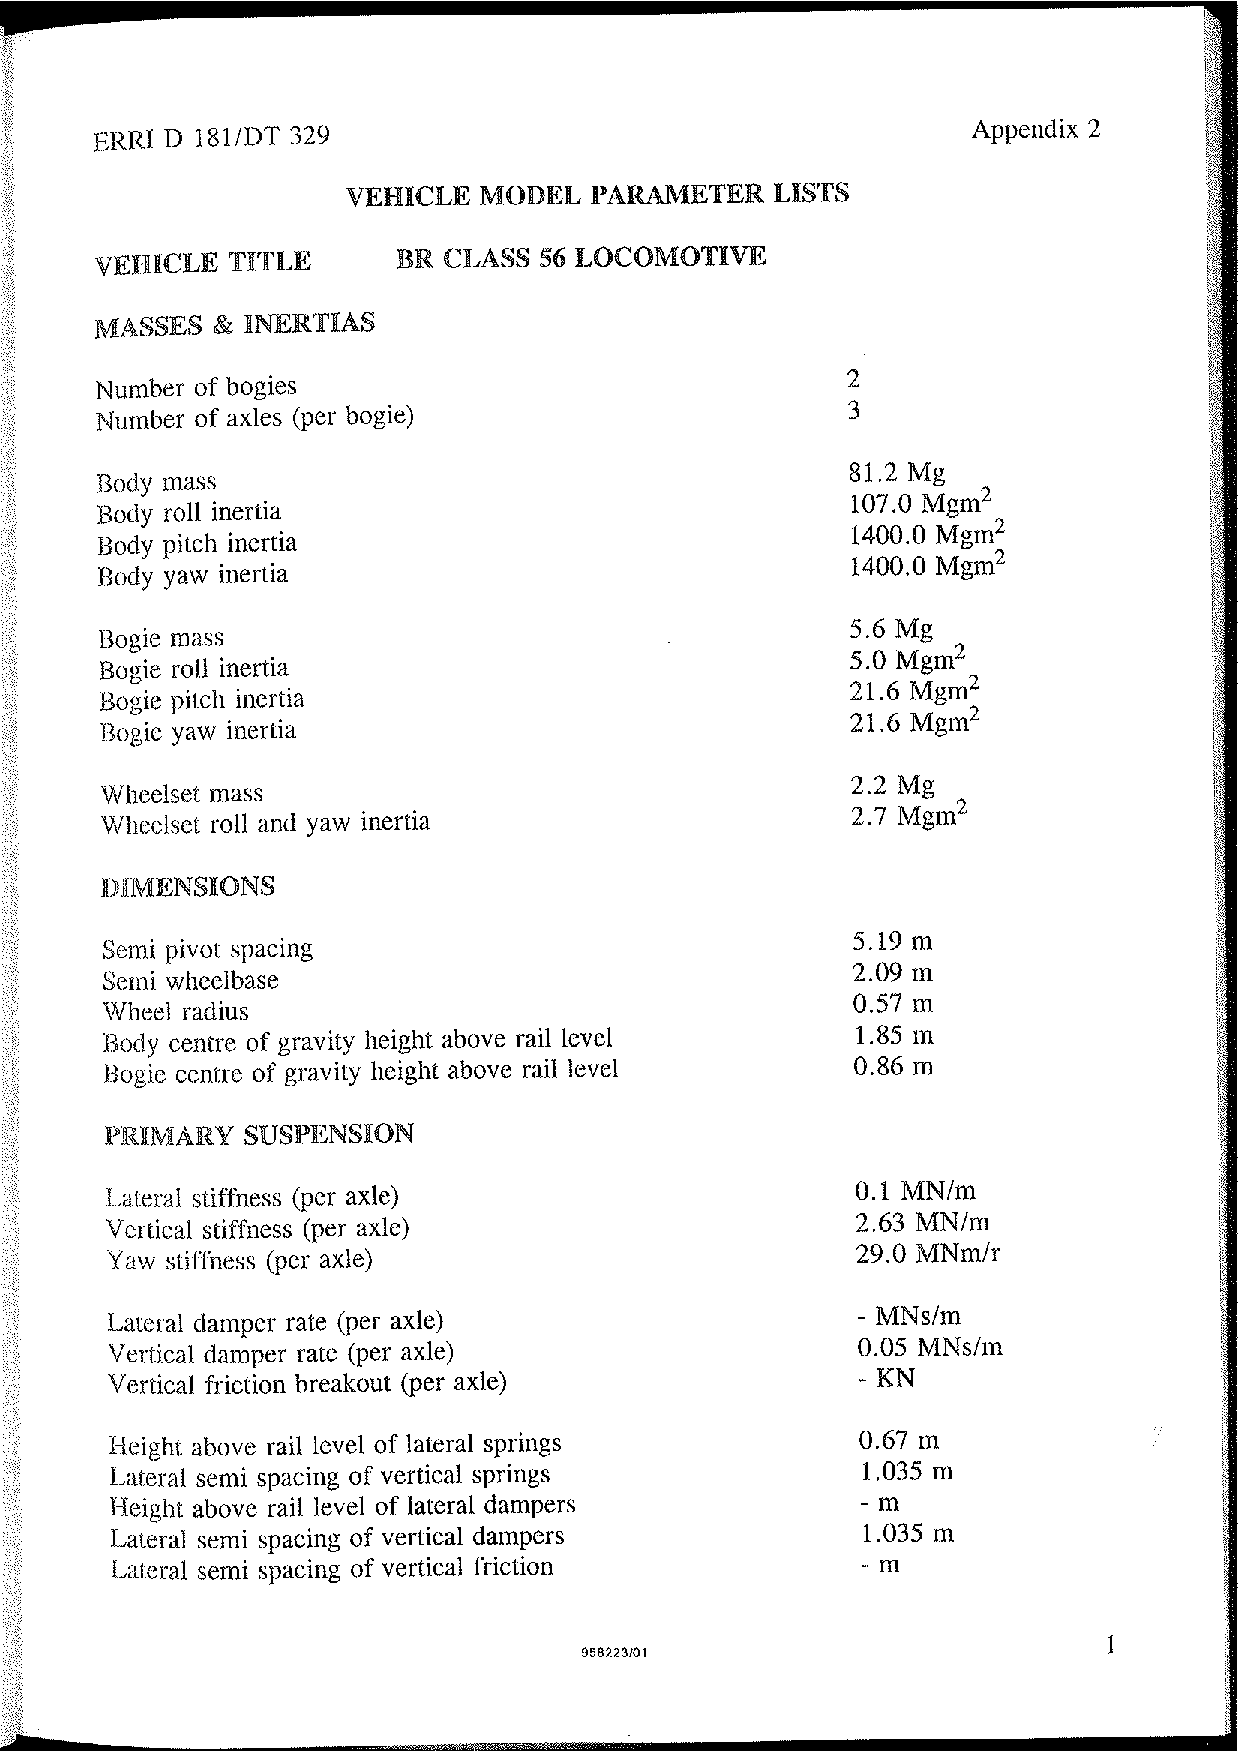
\includegraphics[width=\textwidth]{vp11}
    \caption{BR CLASS 56 LOCOMOTIVE. Extract from \cite[Appendix 2]{d181dt329}}
\end{figure}

\begin{figure}[h]
    \centering
    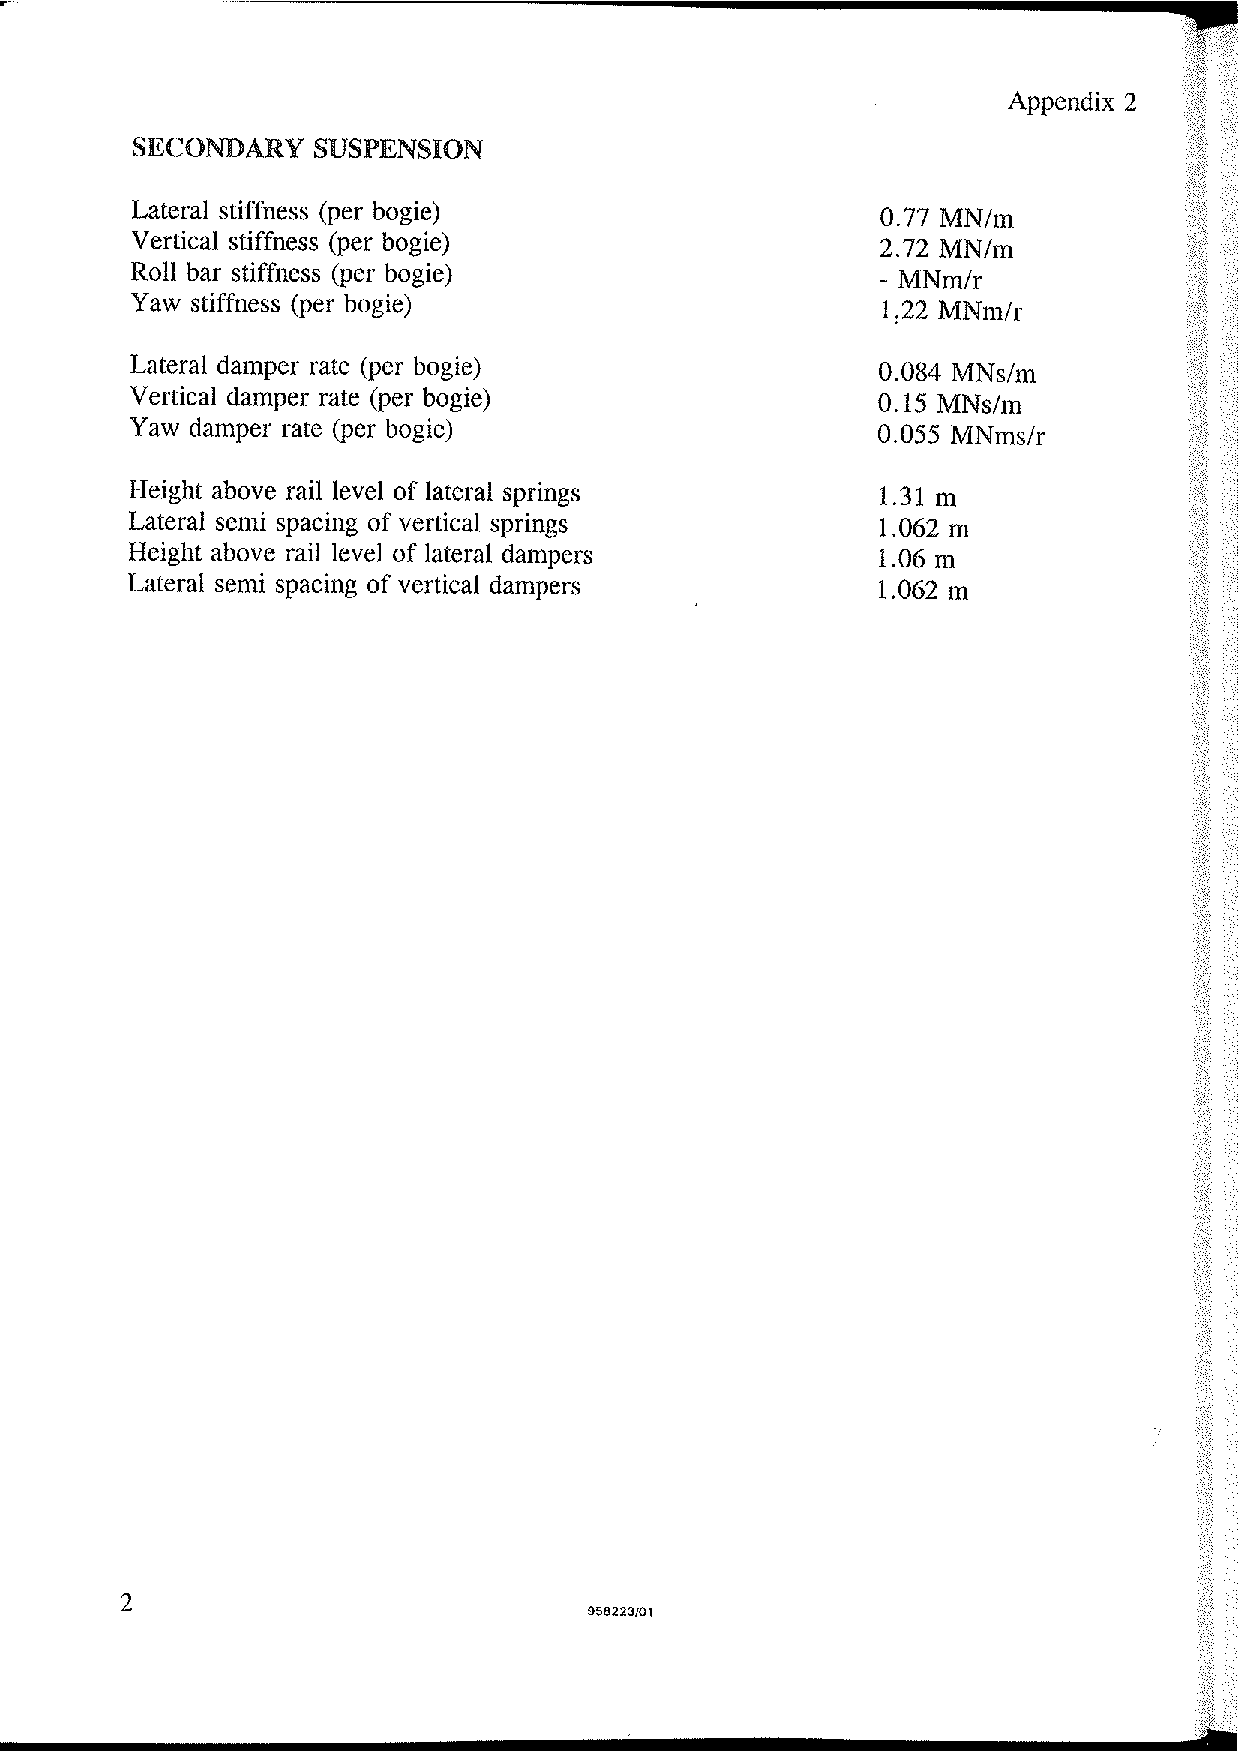
\includegraphics[width=\textwidth]{vp12}
    \caption{BR CLASS 56 LOCOMOTIVE. Extract from \cite[Appendix 2]{d181dt329}}
\end{figure}

\begin{figure}[h]
    \centering
    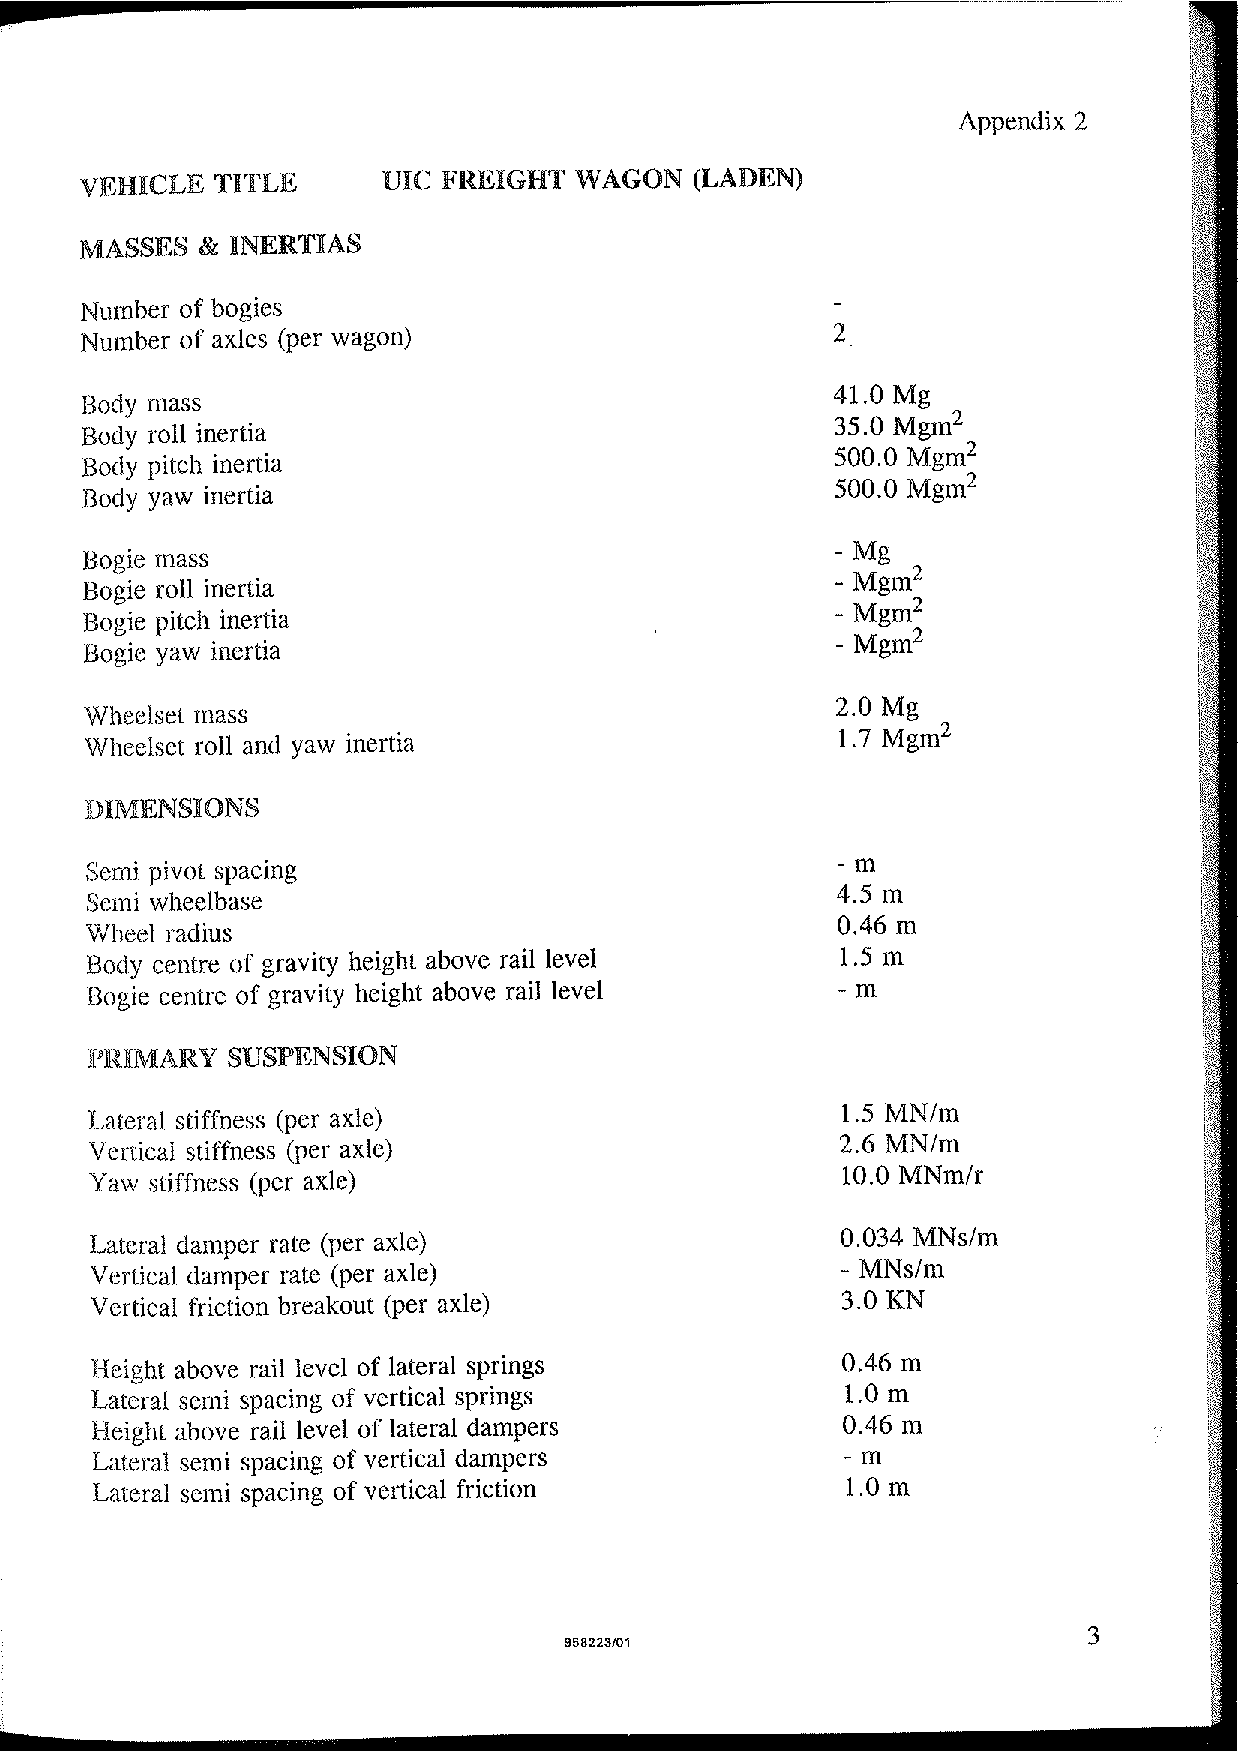
\includegraphics[width=\textwidth]{vp21}
    \caption{UIC FREIGHT WAGON (LADEN). Extract from \cite[Appendix 2]{d181dt329}}
\end{figure}

\begin{figure}[h]
    \centering
    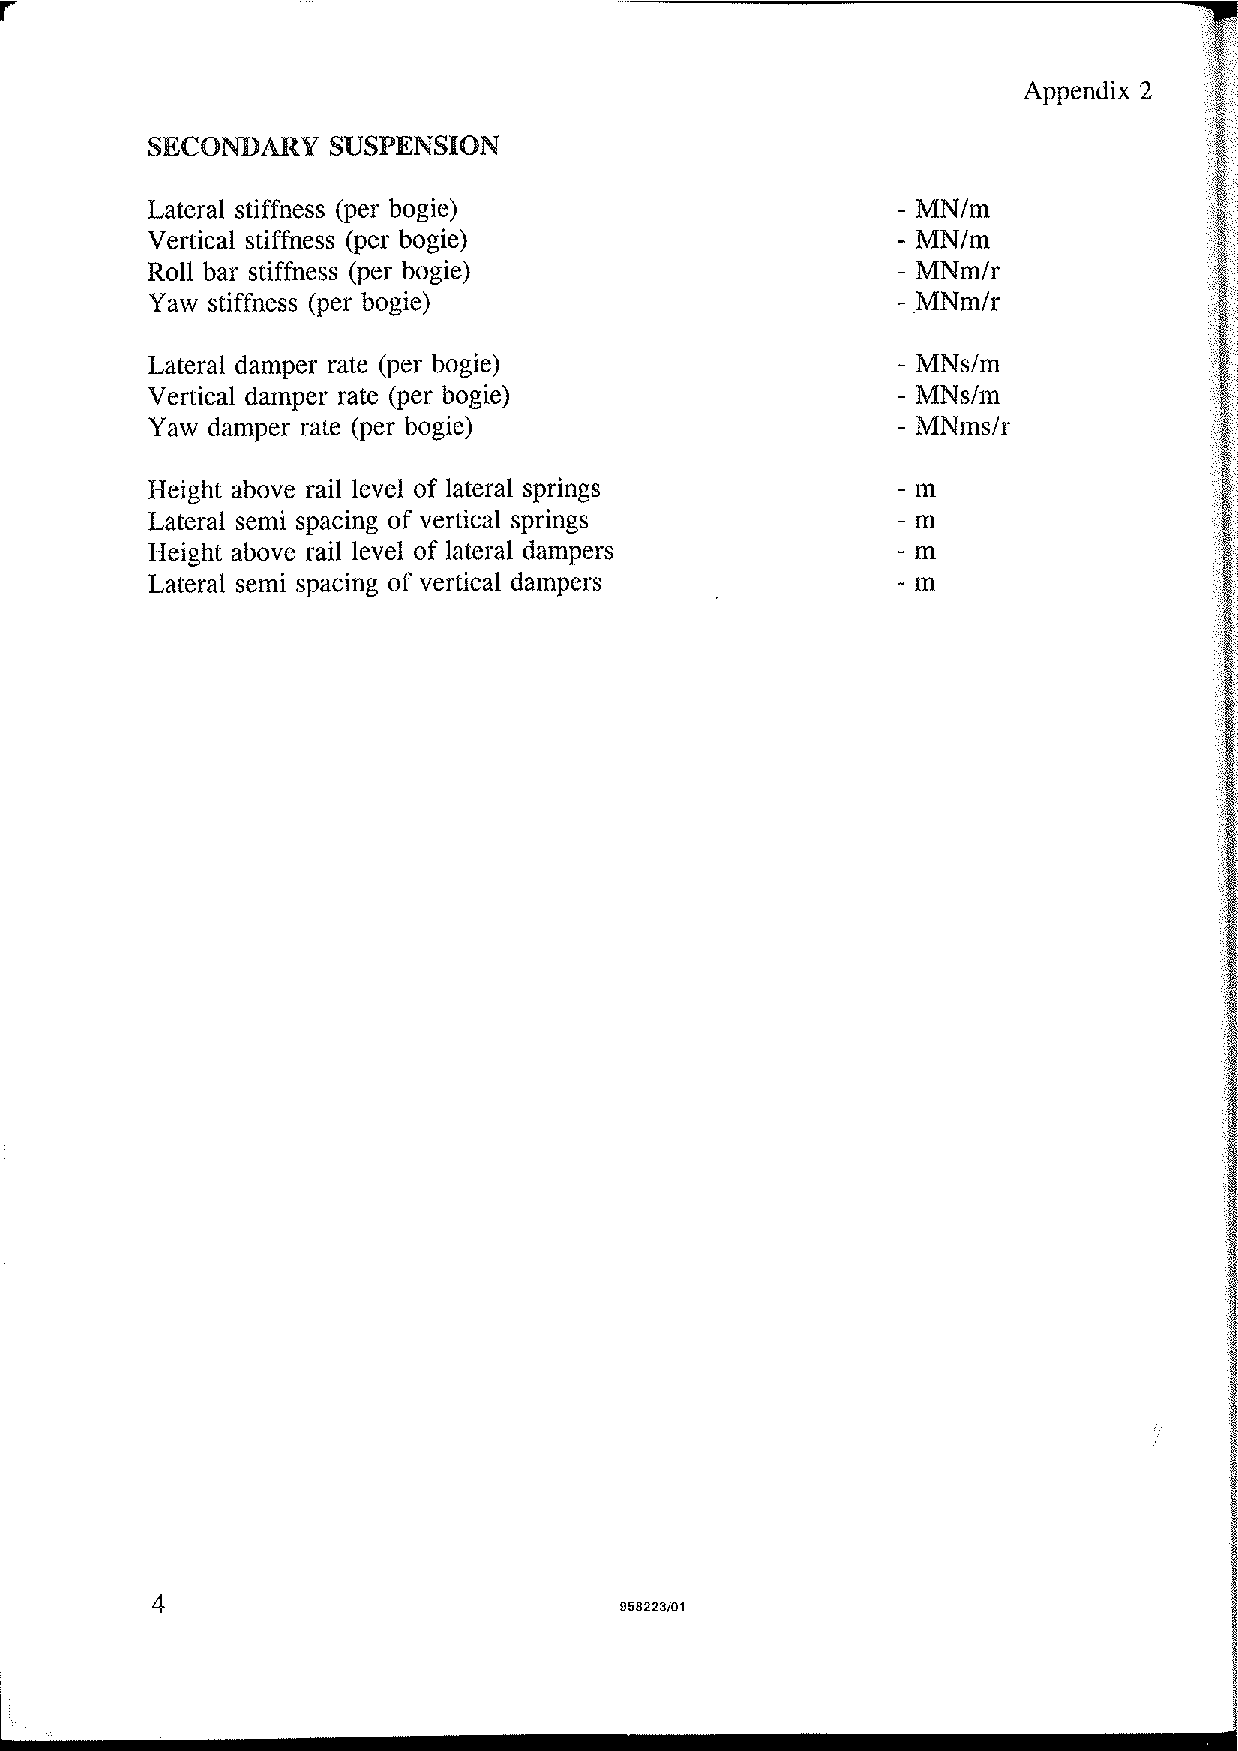
\includegraphics[width=\textwidth]{vp22}
    \caption{UIC FREIGHT WAGON (LADEN). Extract from \cite[Appendix 2]{d181dt329}}
\end{figure}

\begin{figure}[h]
    \centering
    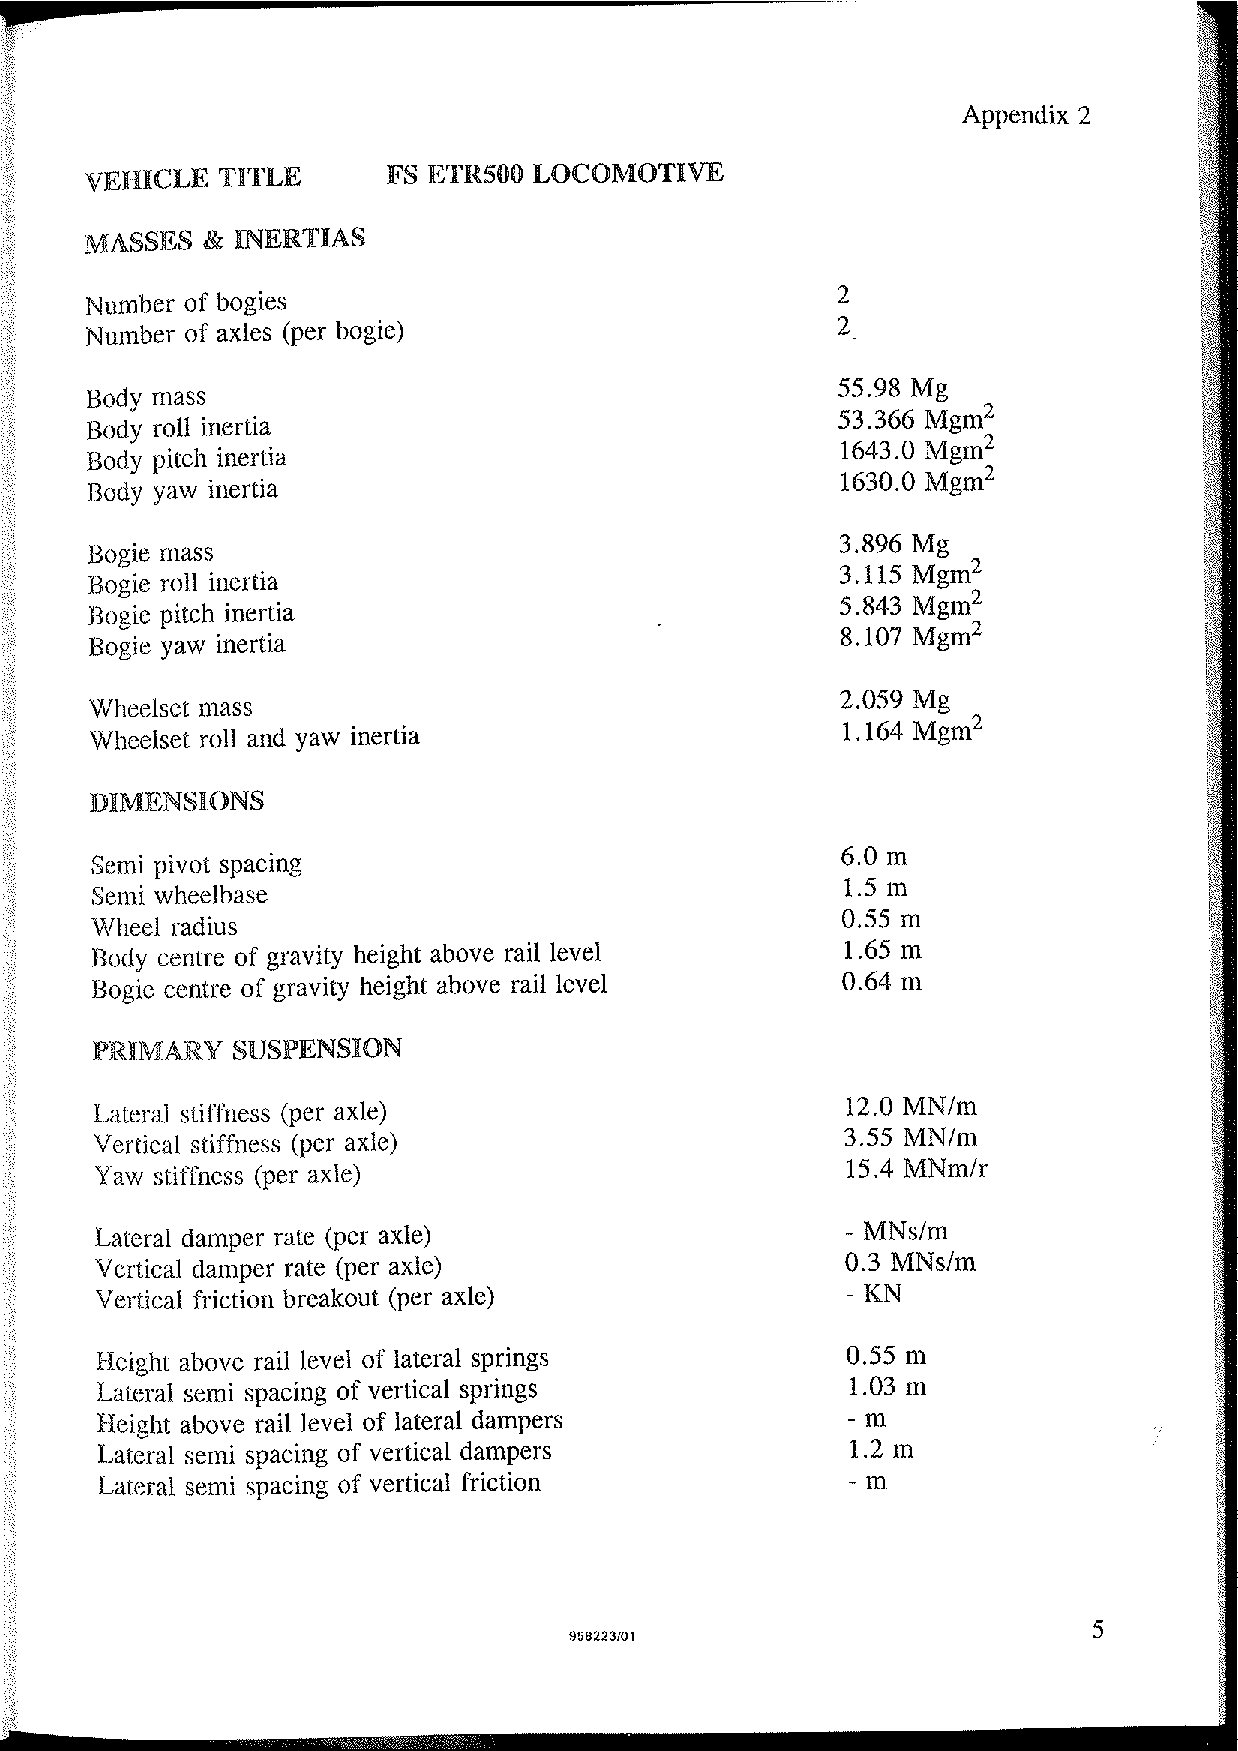
\includegraphics[width=\textwidth]{vp31}
    \caption{FS ETR500 LOCOMOTIVE. Extract from \cite[Appendix 2]{d181dt329}}
\end{figure}

\begin{figure}[h]
    \centering
    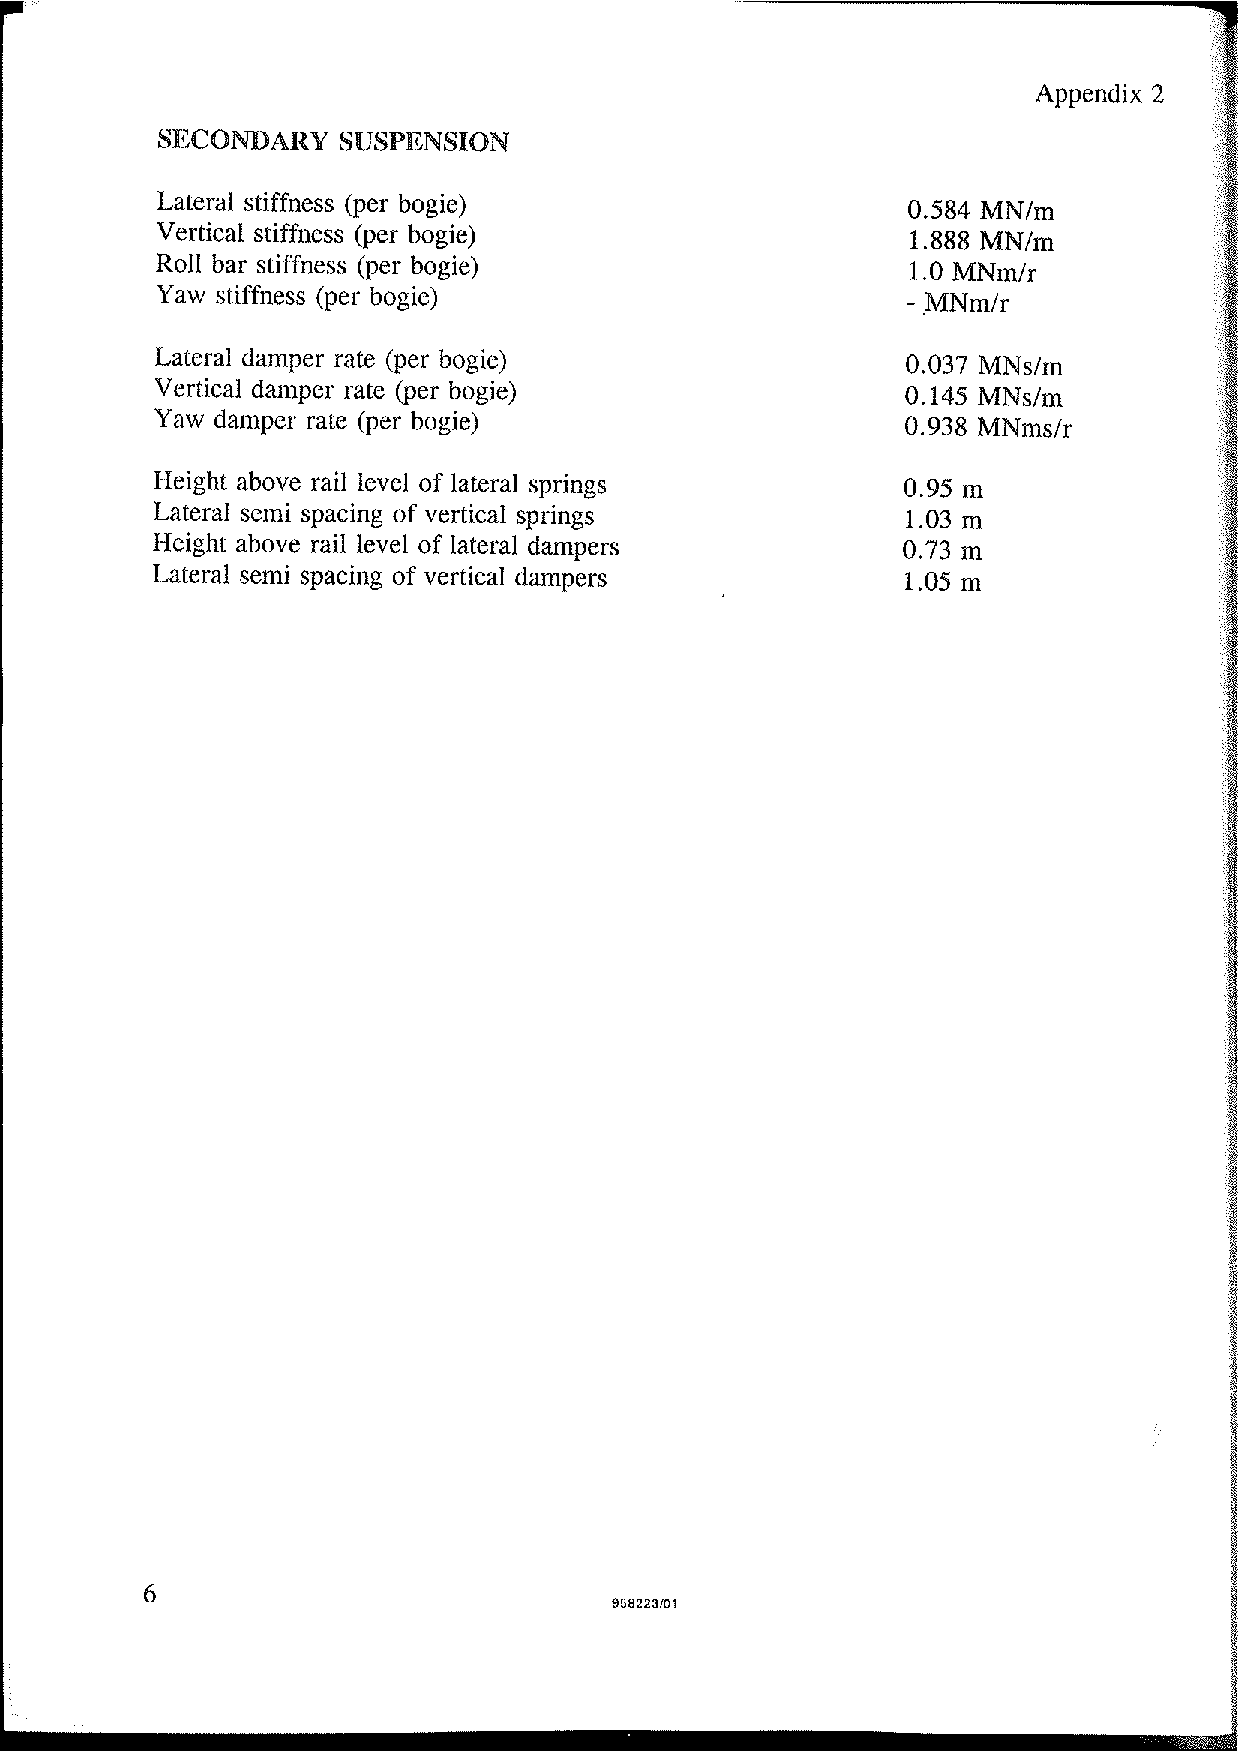
\includegraphics[width=\textwidth]{vp32}
    \caption{FS ETR500 LOCOMOTIVE. Extract from \cite[Appendix 2]{d181dt329}}
\end{figure}

\begin{figure}[h]
    \centering
    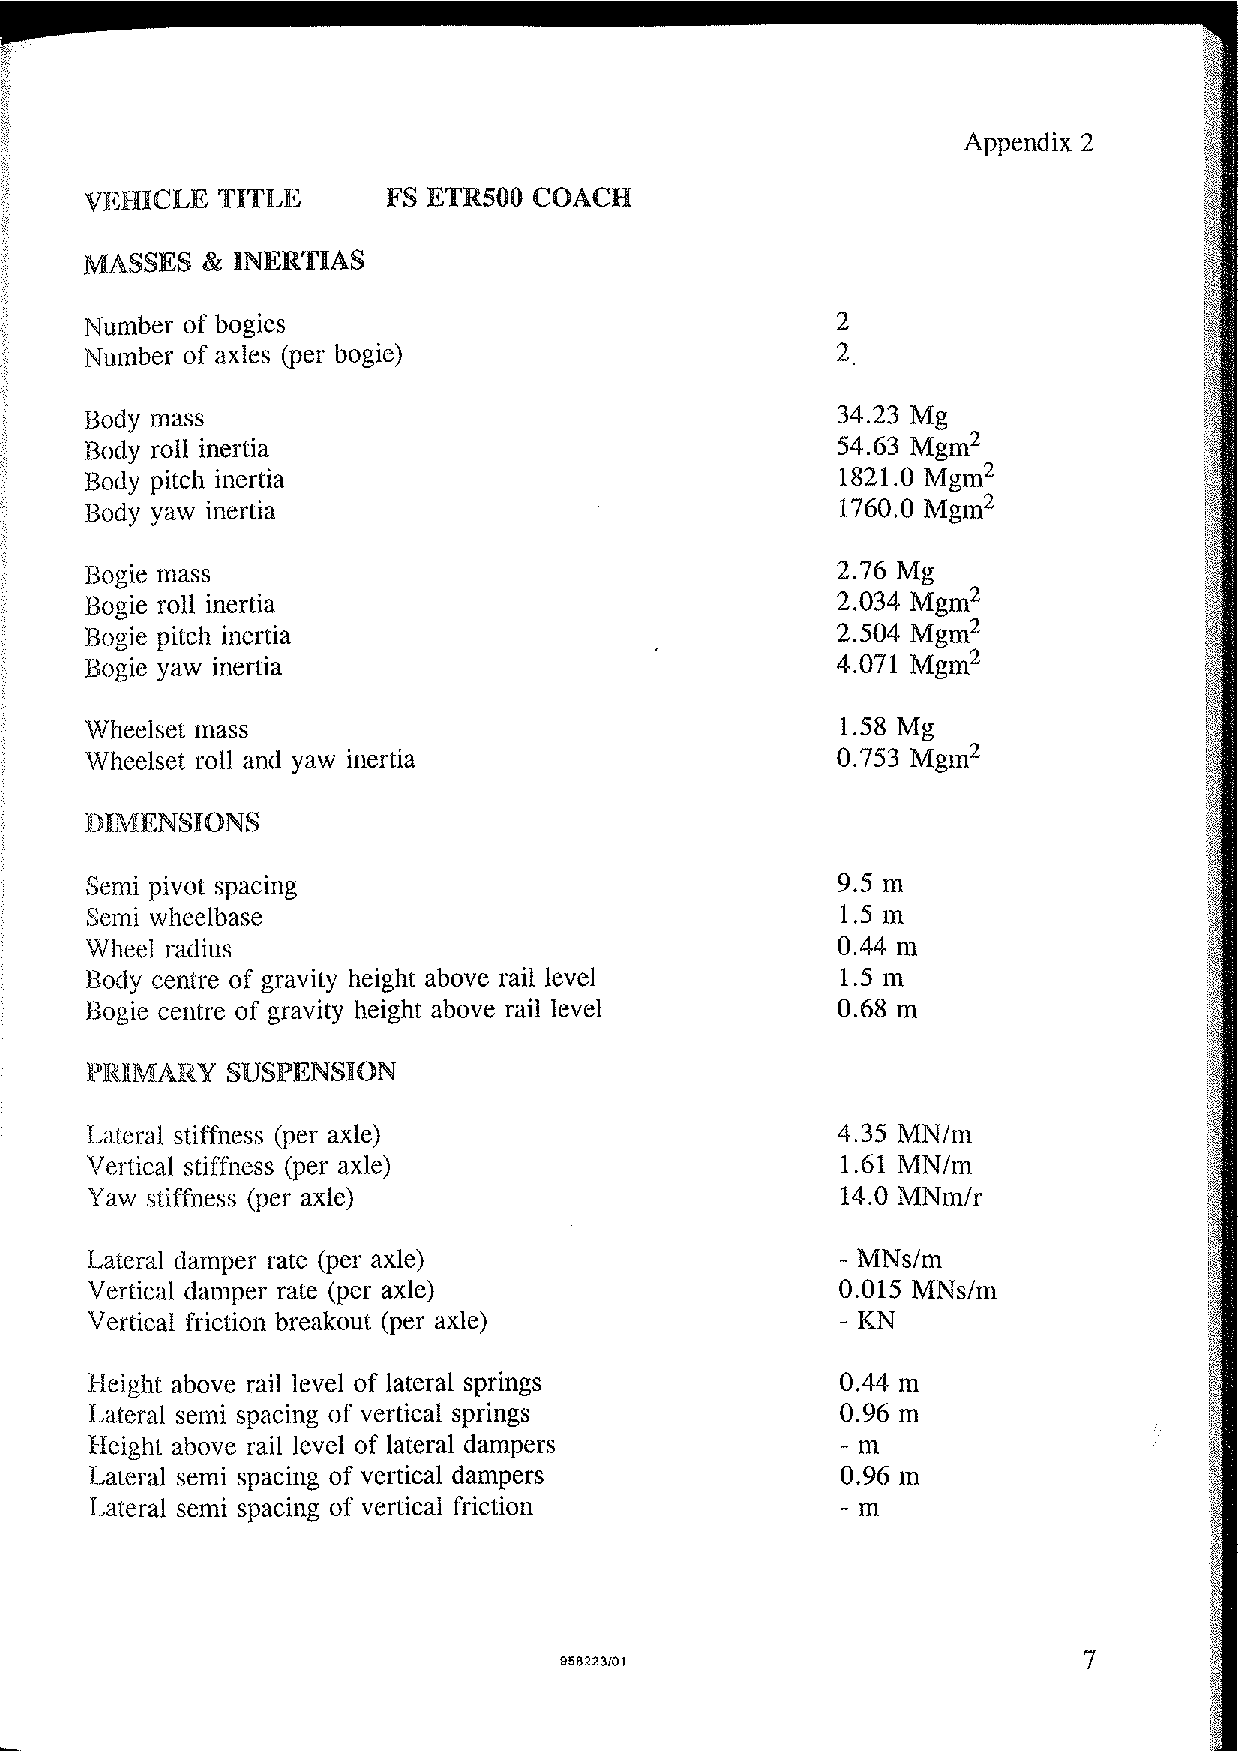
\includegraphics[width=\textwidth]{vp41}
    \caption{FS ETR500 COACH. Extract from \cite[Appendix 2]{d181dt329}}
\end{figure}

\begin{figure}[h]
    \centering
    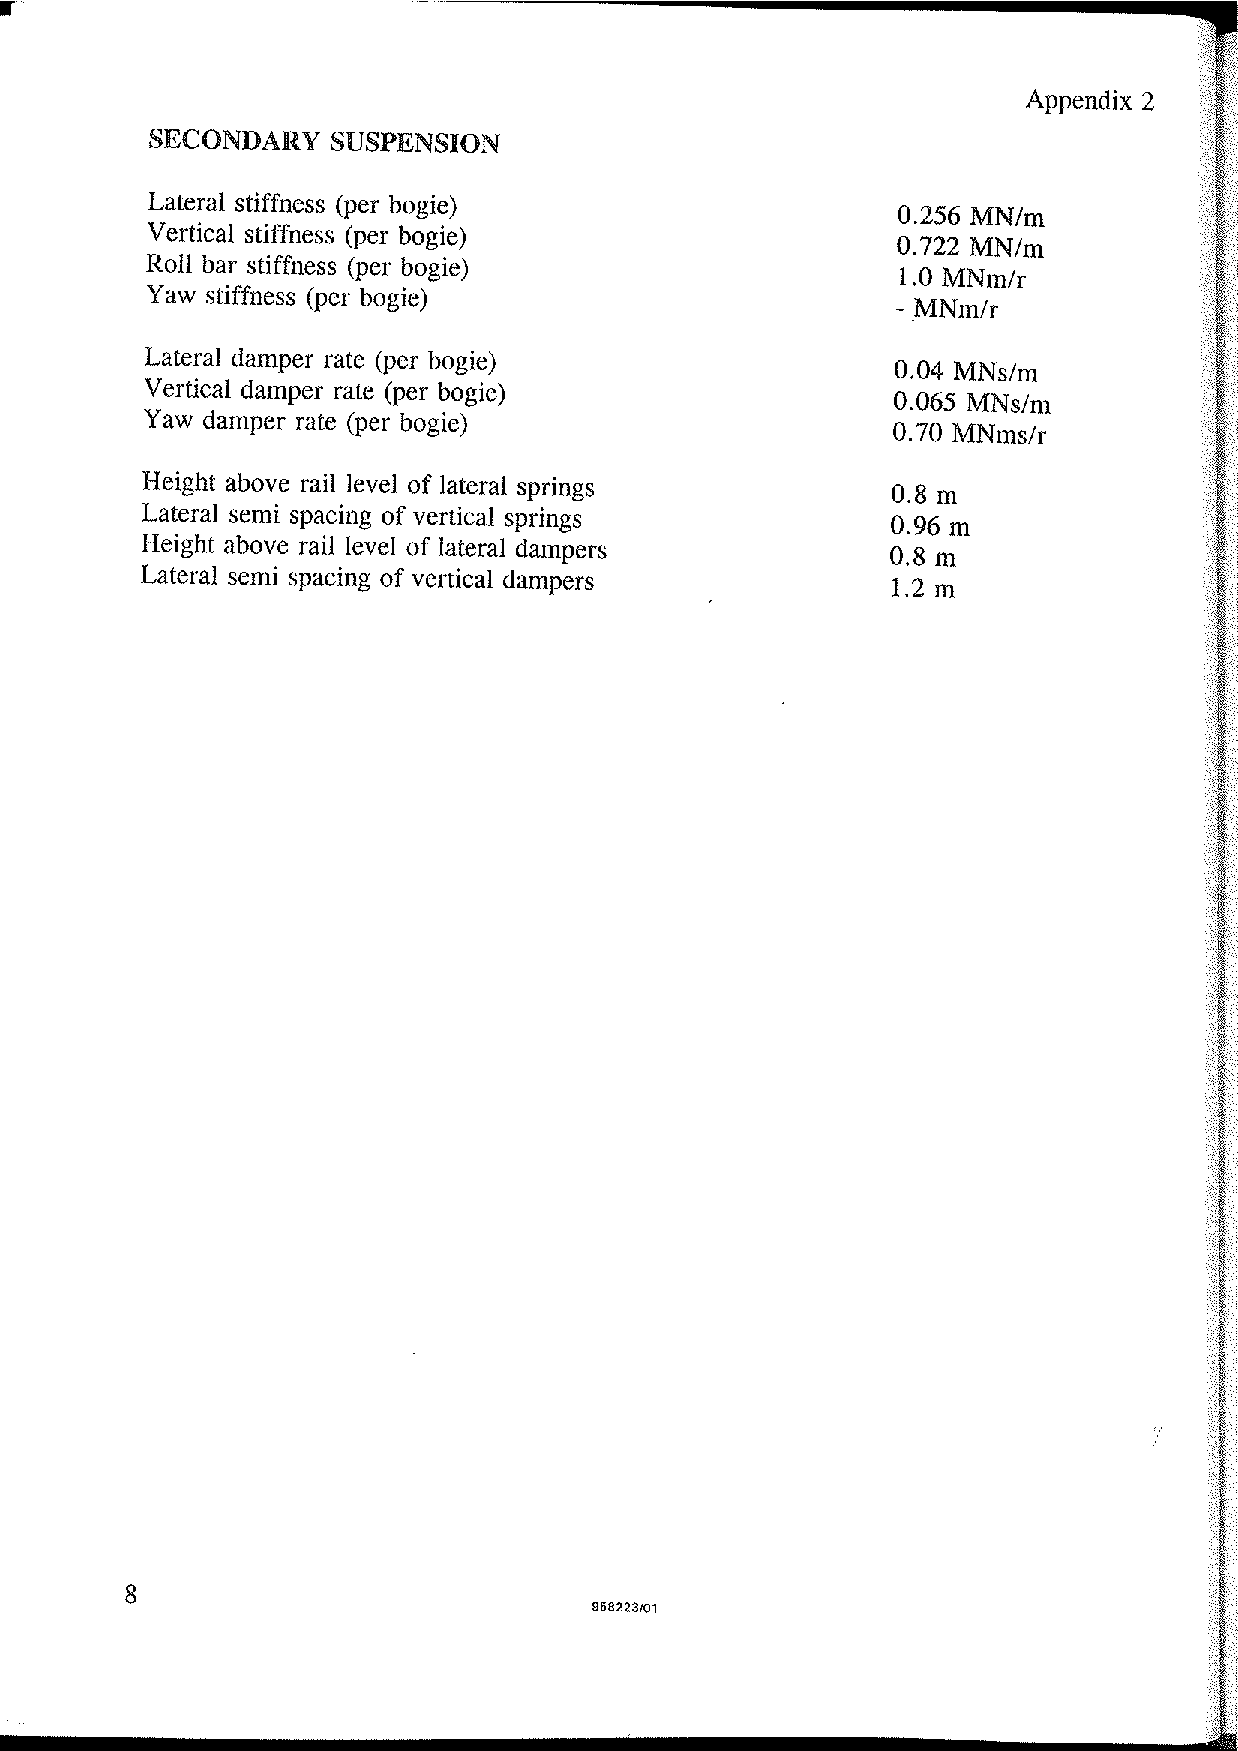
\includegraphics[width=\textwidth]{vp42}
    \caption{FS ETR500 COACH. Extract from \cite[Appendix 2]{d181dt329}}
\end{figure}

\begin{figure}[h]
    \centering
    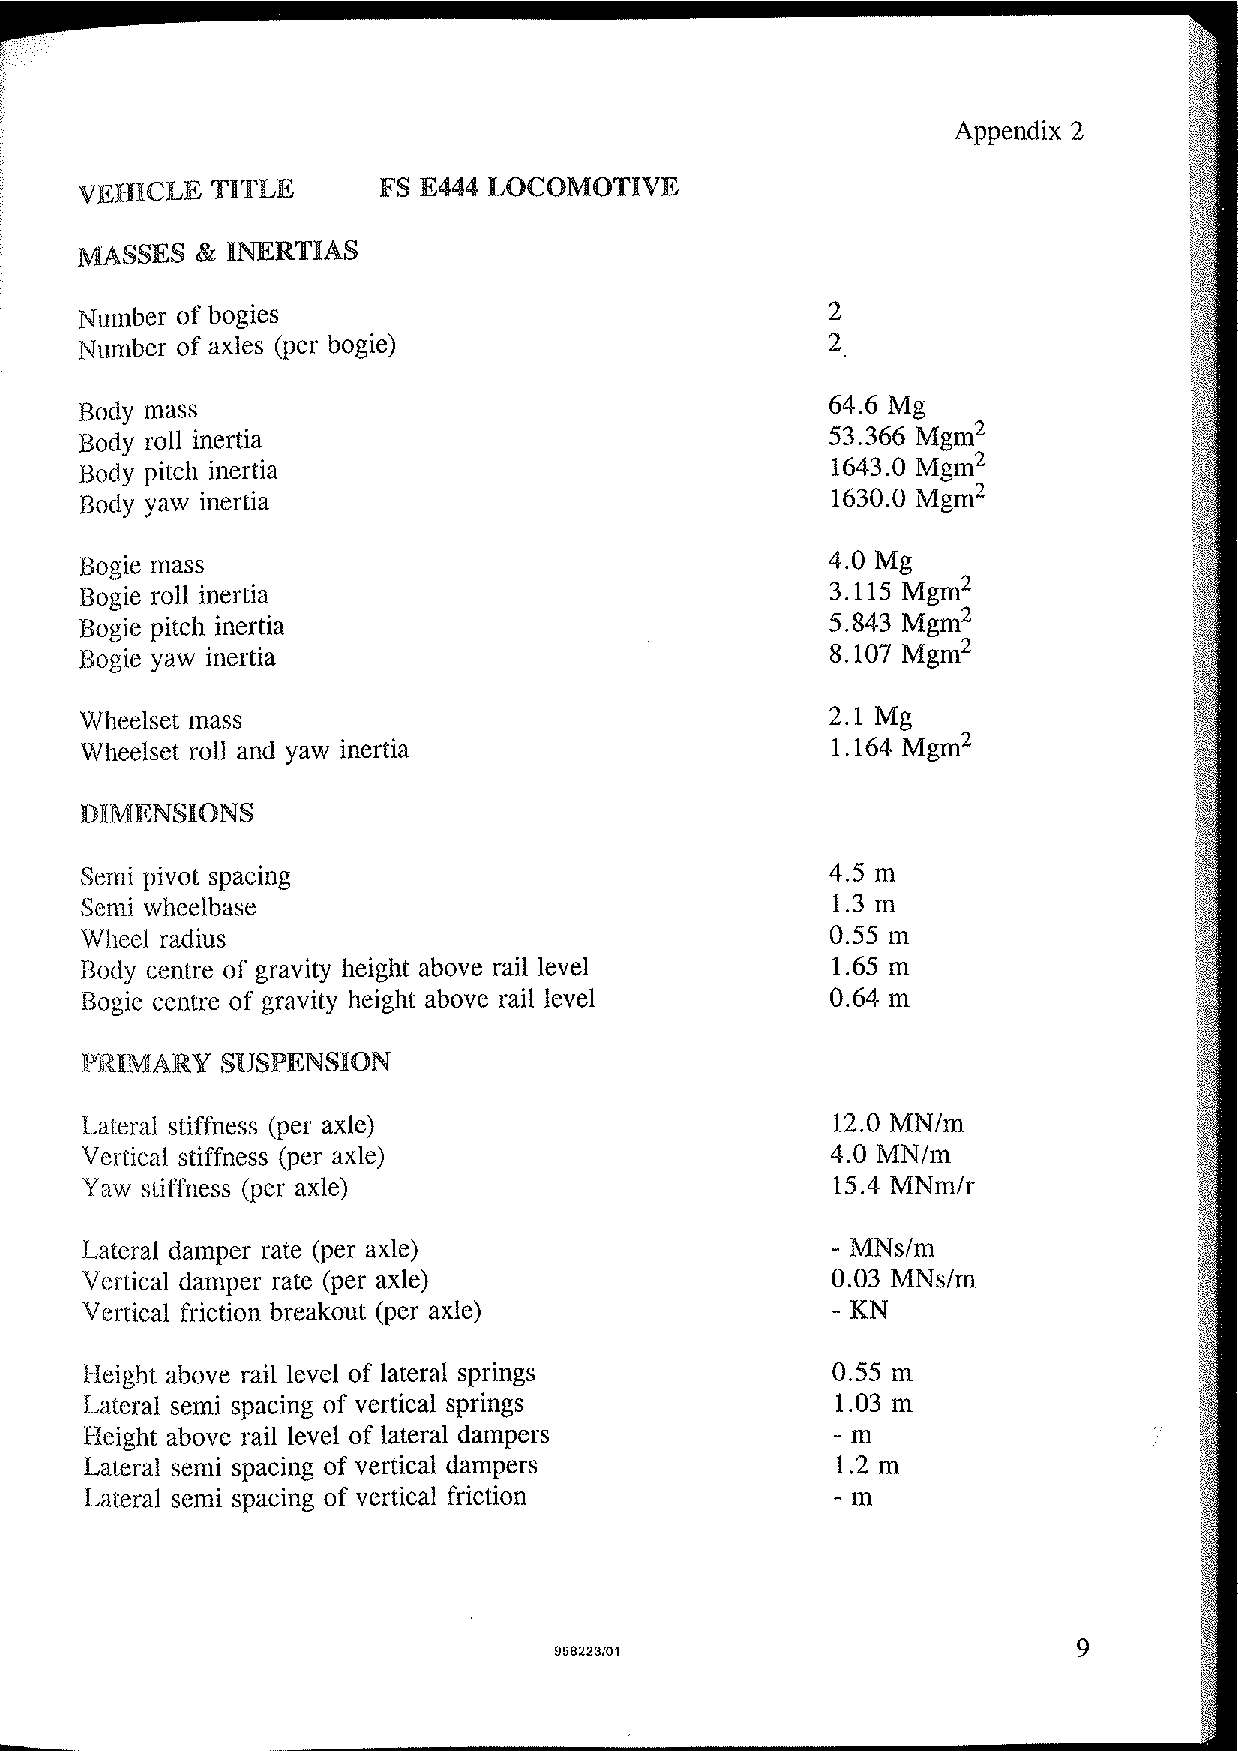
\includegraphics[width=\textwidth]{vp51}
    \caption{FS E444 LOCOMOTIVE. Extract from \cite[Appendix 2]{d181dt329}}
\end{figure}

\begin{figure}[h]
    \centering
    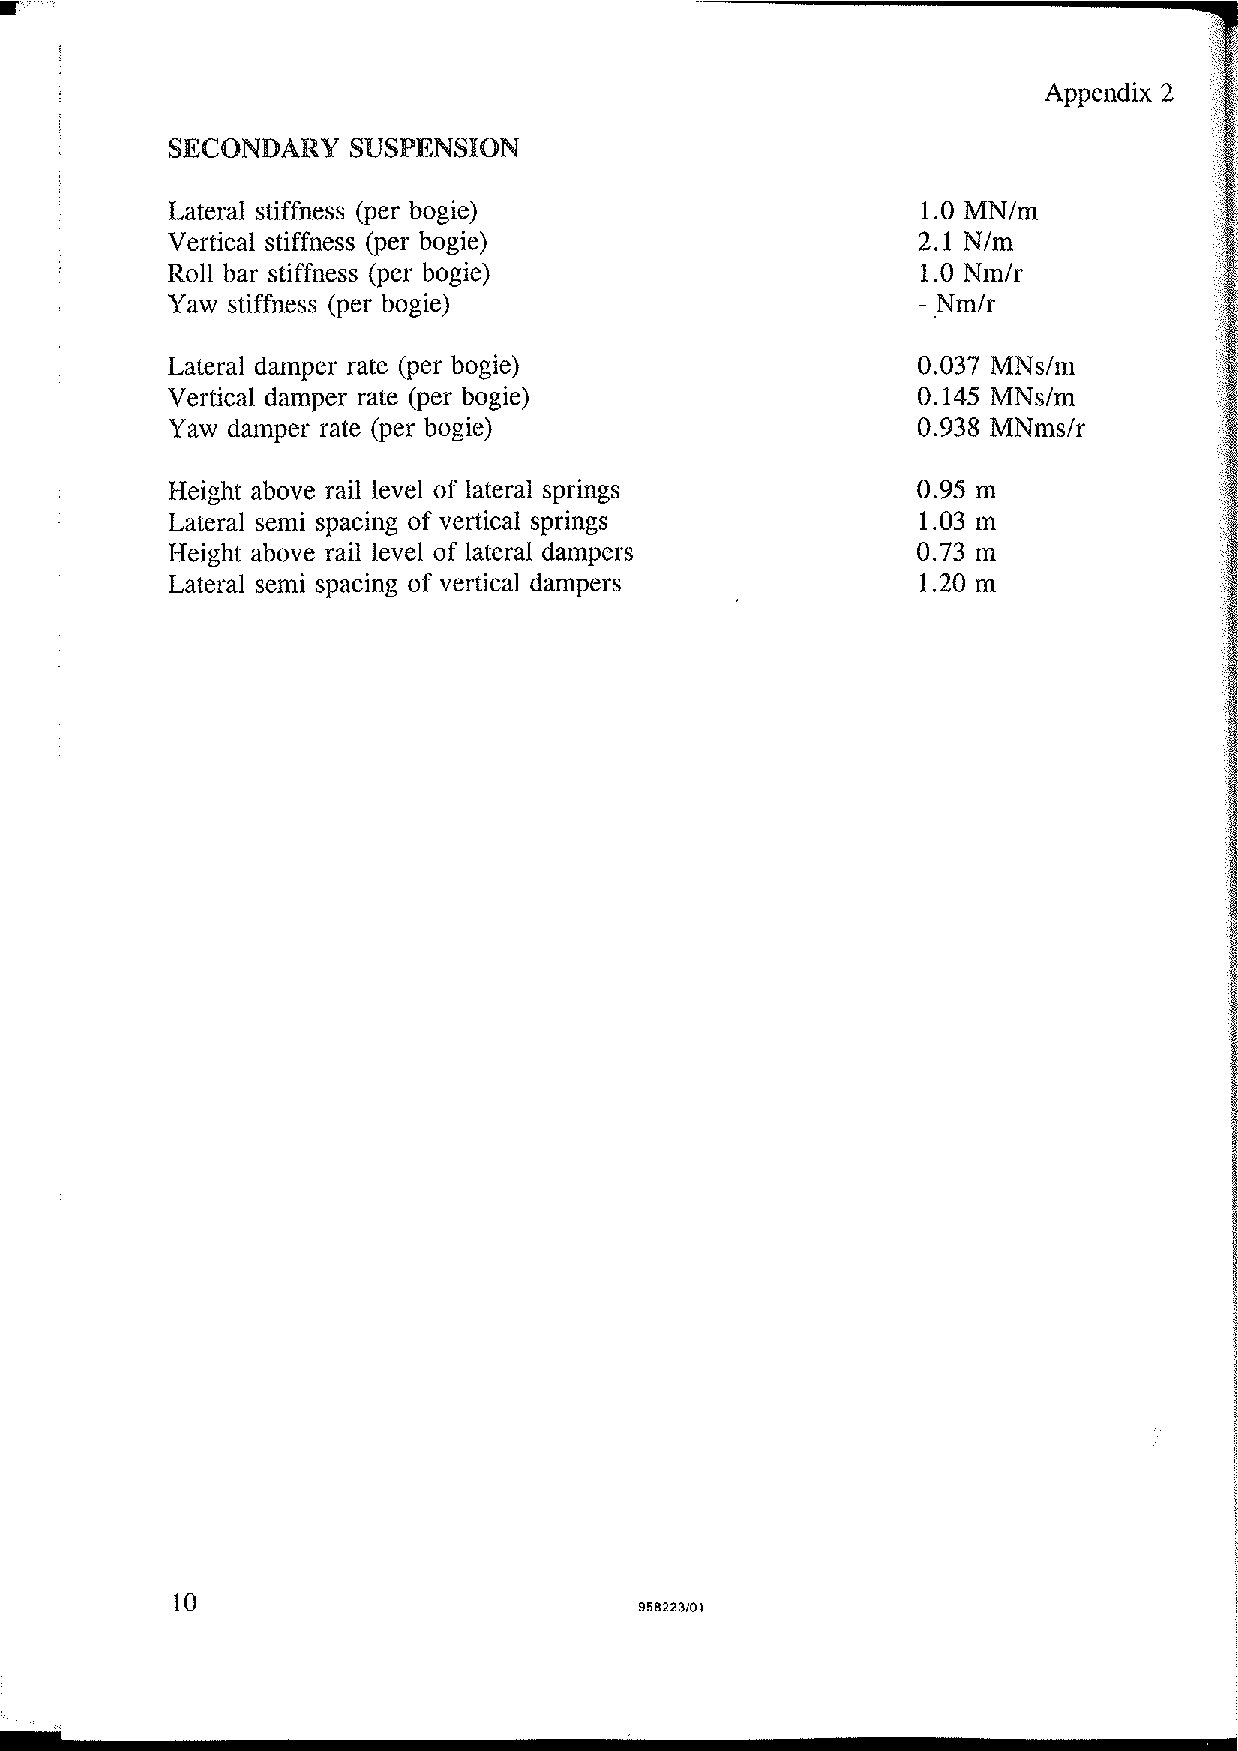
\includegraphics[width=\textwidth]{vp52}
    \caption{FS E444 LOCOMOTIVE. Extract from \cite[Appendix 2]{d181dt329}}
\end{figure}

\begin{figure}[h]
    \centering
    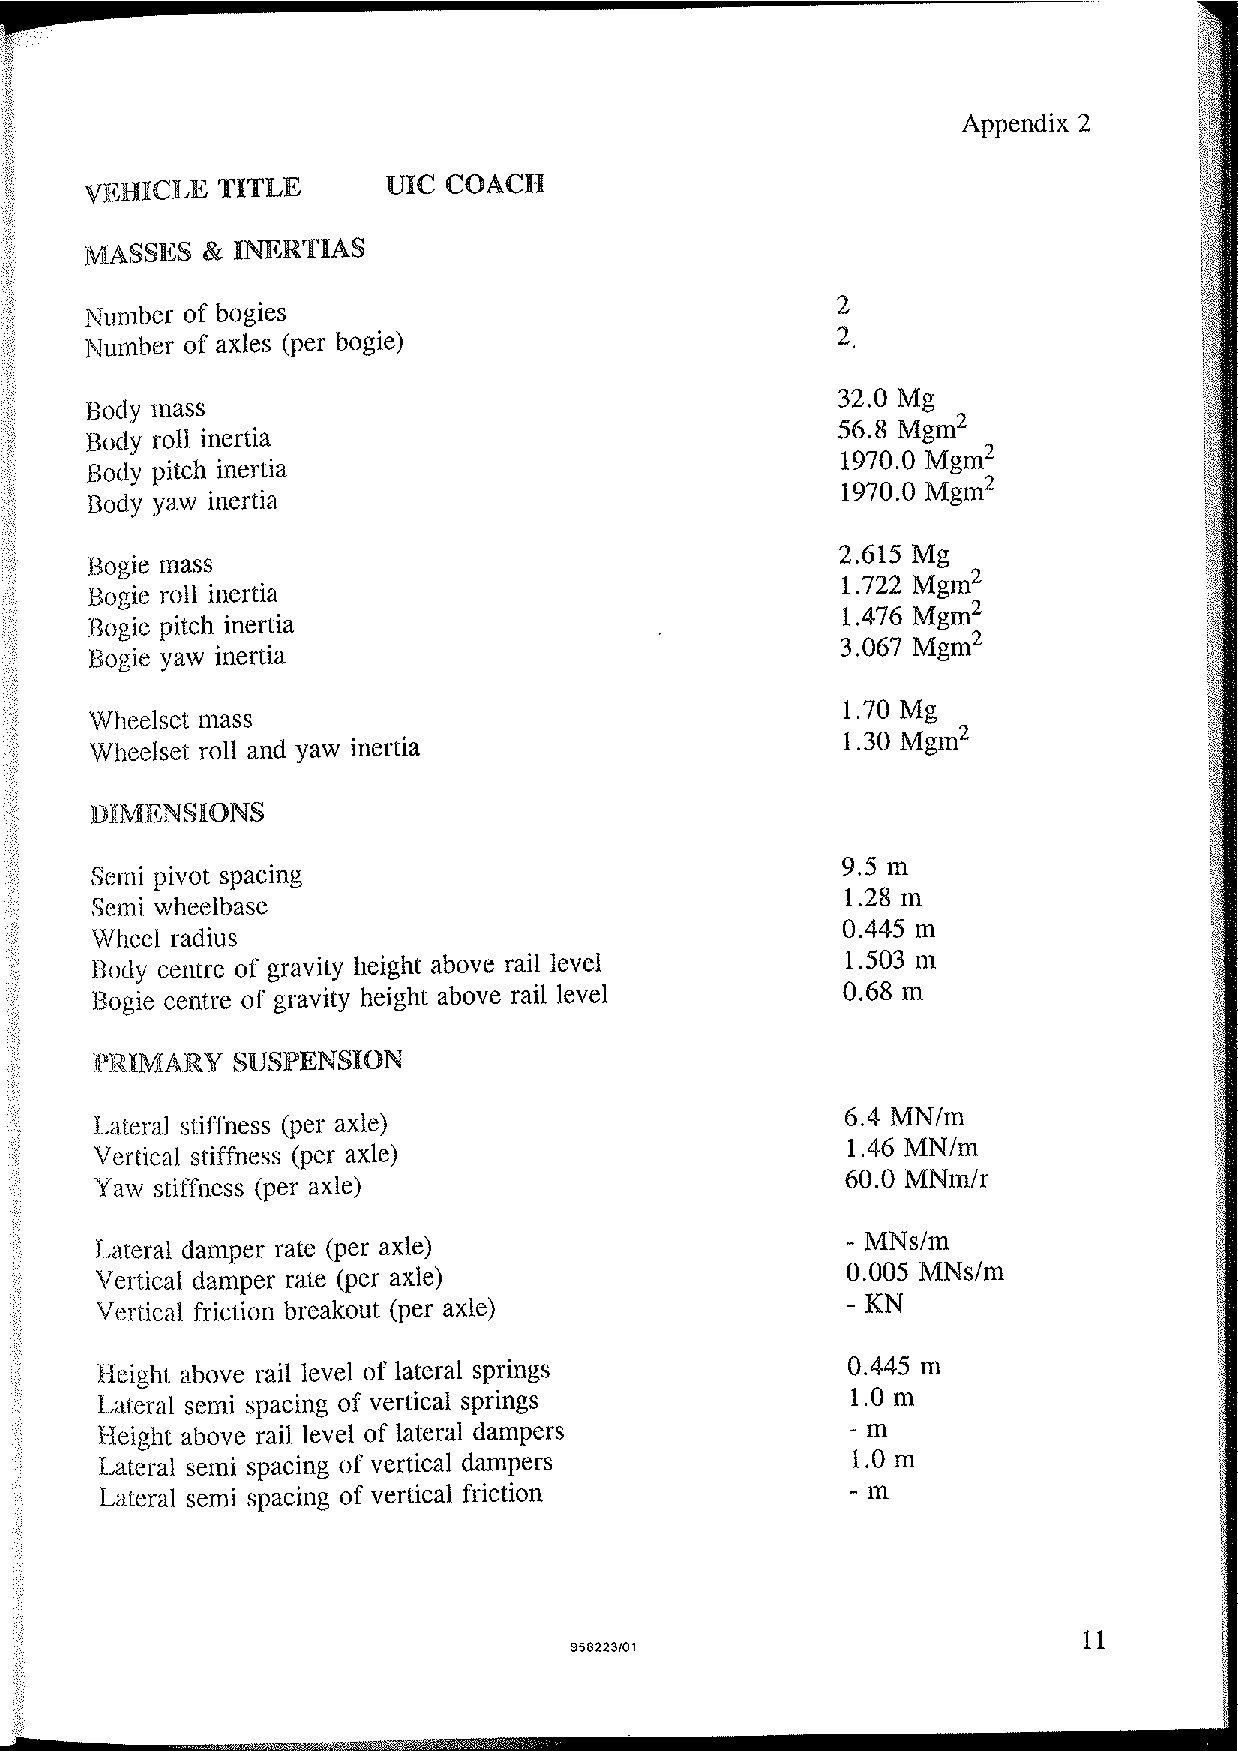
\includegraphics[width=\textwidth]{vp61}
    \caption{UIC COACH. Extract from \cite[Appendix 2]{d181dt329}}
\end{figure}

\begin{figure}[h]
    \centering
    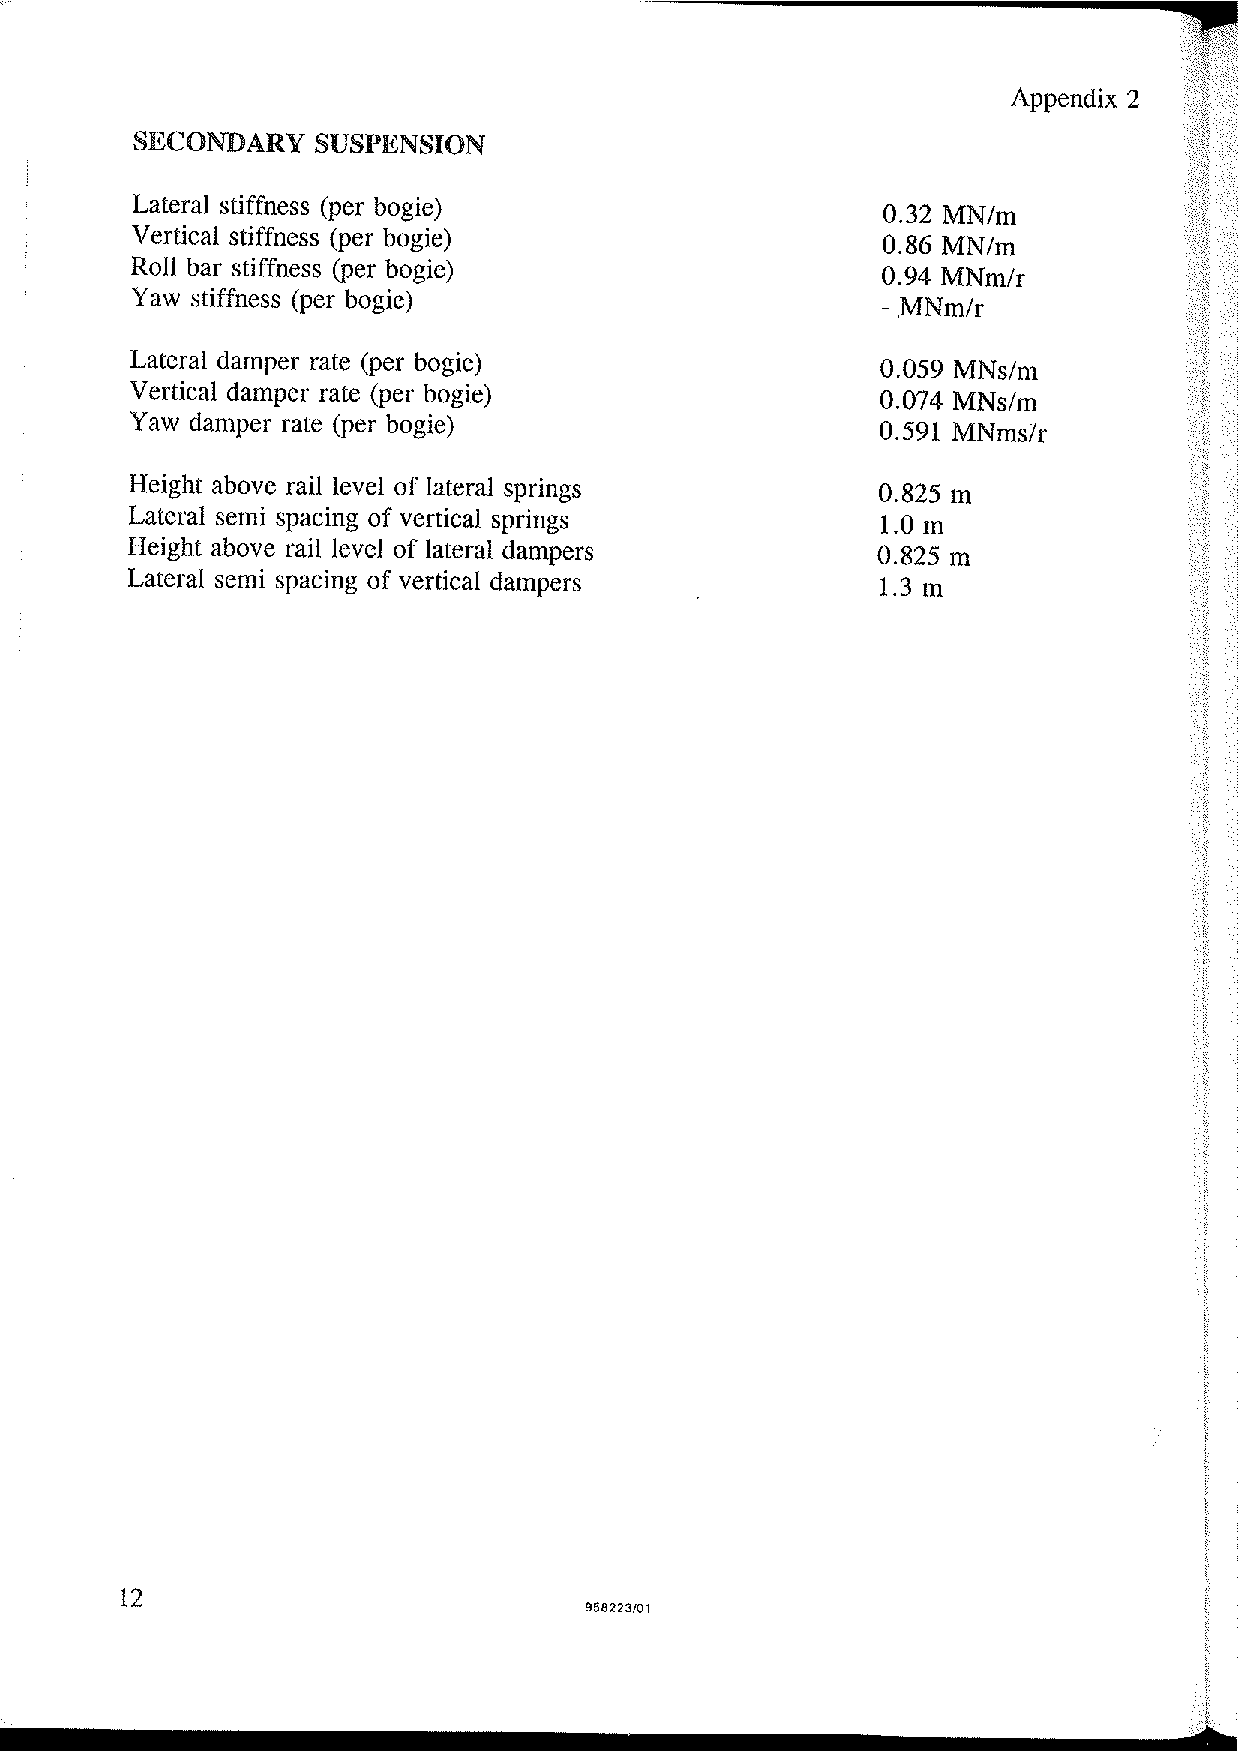
\includegraphics[width=\textwidth]{vp62}
    \caption{UIC COACH. Extract from \cite[Appendix 2]{d181dt329}}
\end{figure}

\begin{figure}[h]    \centering
    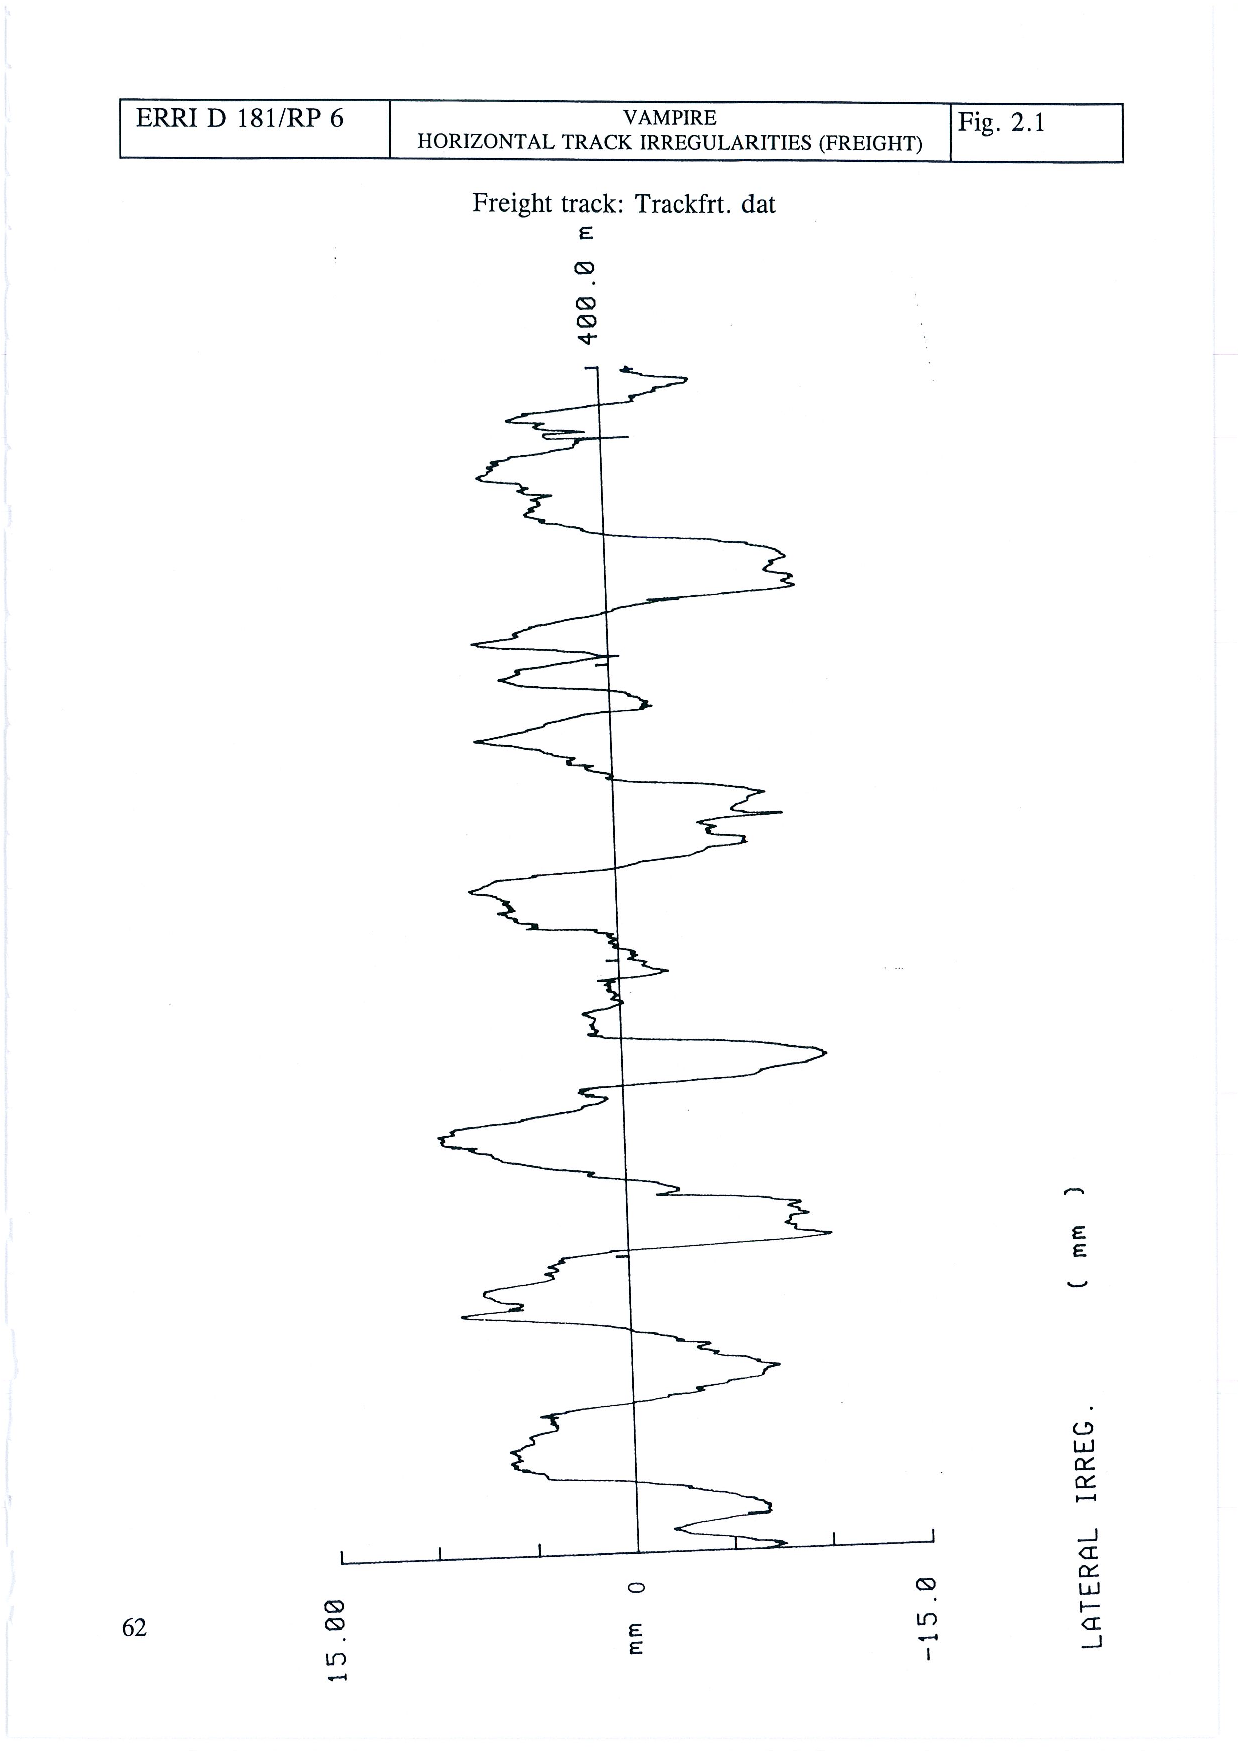
\includegraphics[width=\textwidth]{track1}
    \caption{Horizontal track irregularities for freight trains. Extract from \cite[Figure 2.1]{d181}}
    \label{fig:track1}
\end{figure}

\begin{figure}[h]
    \centering
    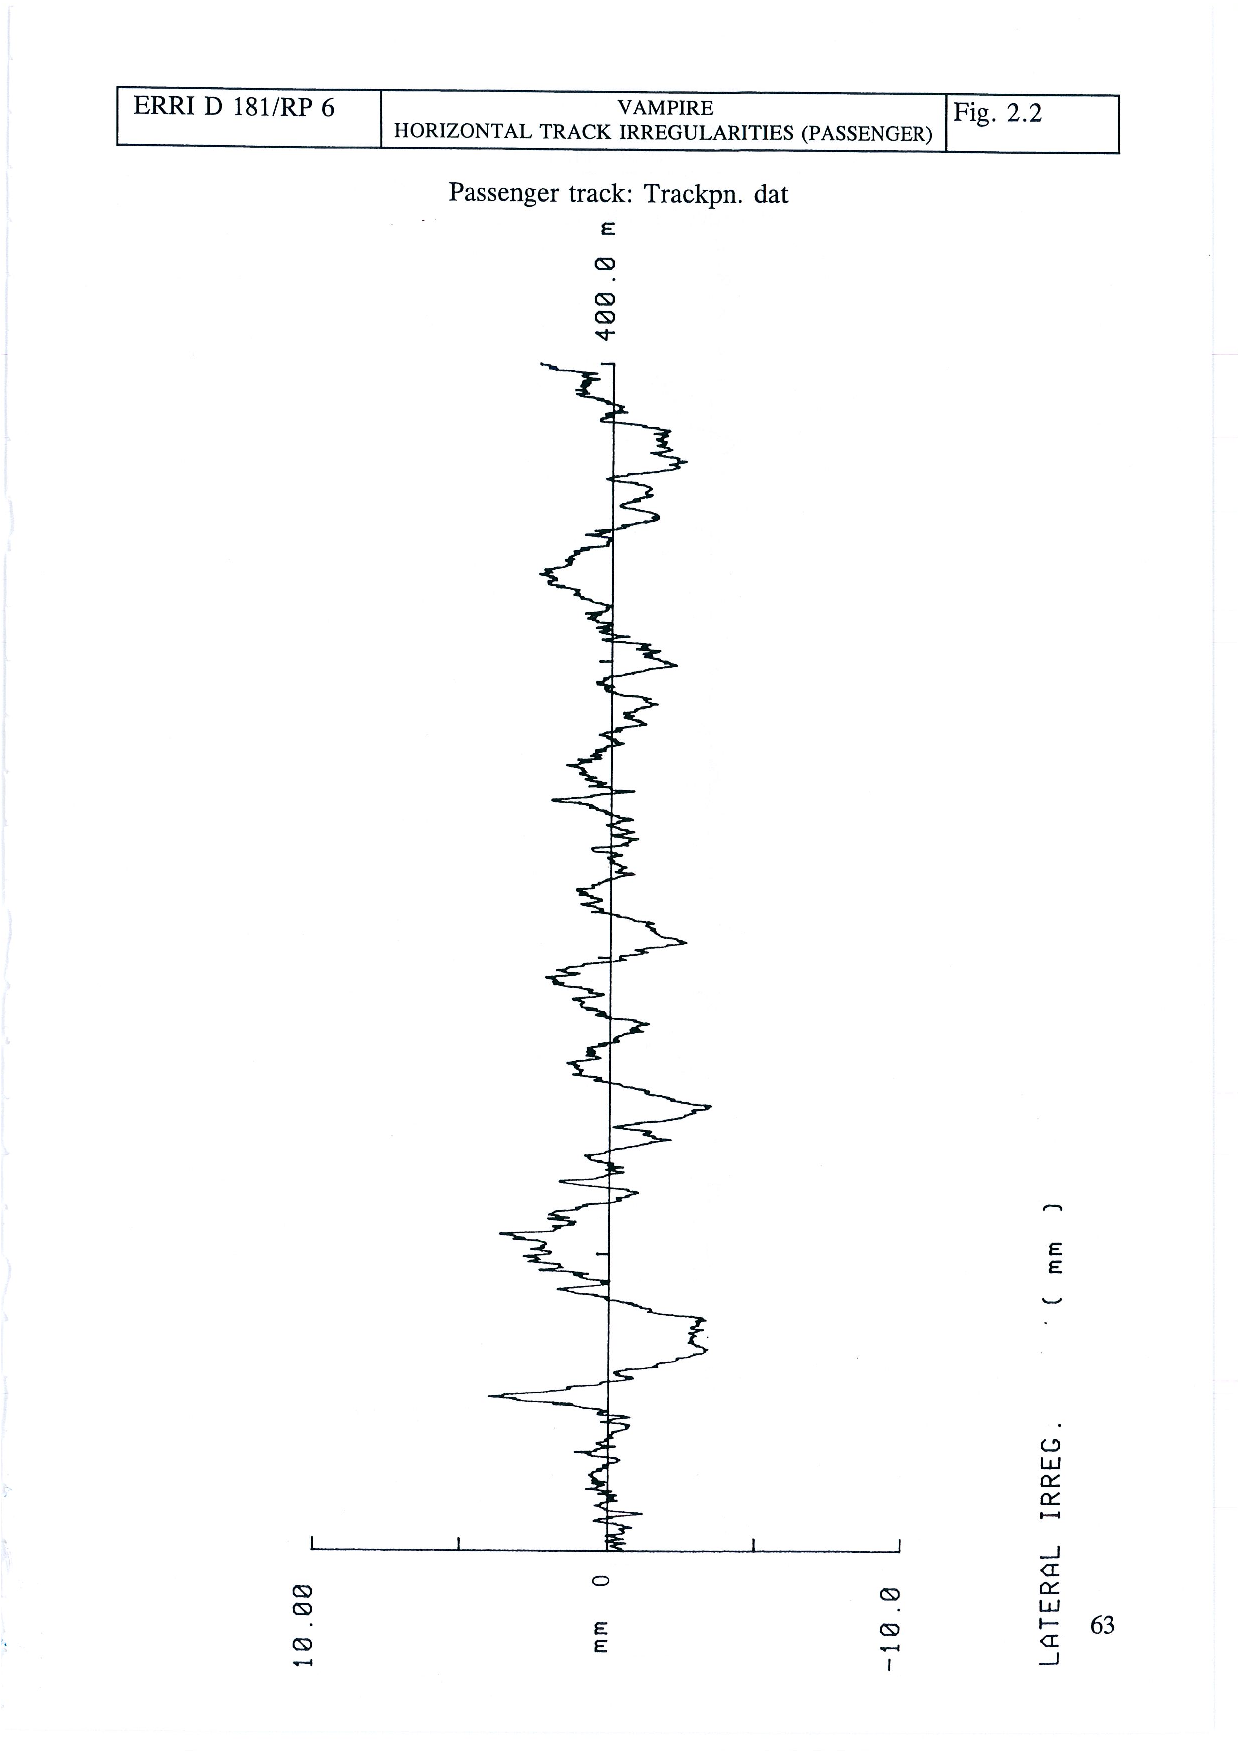
\includegraphics[width=\textwidth]{track2}
    \caption{Horizontal track irregularities for standard passenger trains. Extract from \cite[Figure 2.1]{d181}}
\end{figure}

\begin{figure}[h]
    \centering
    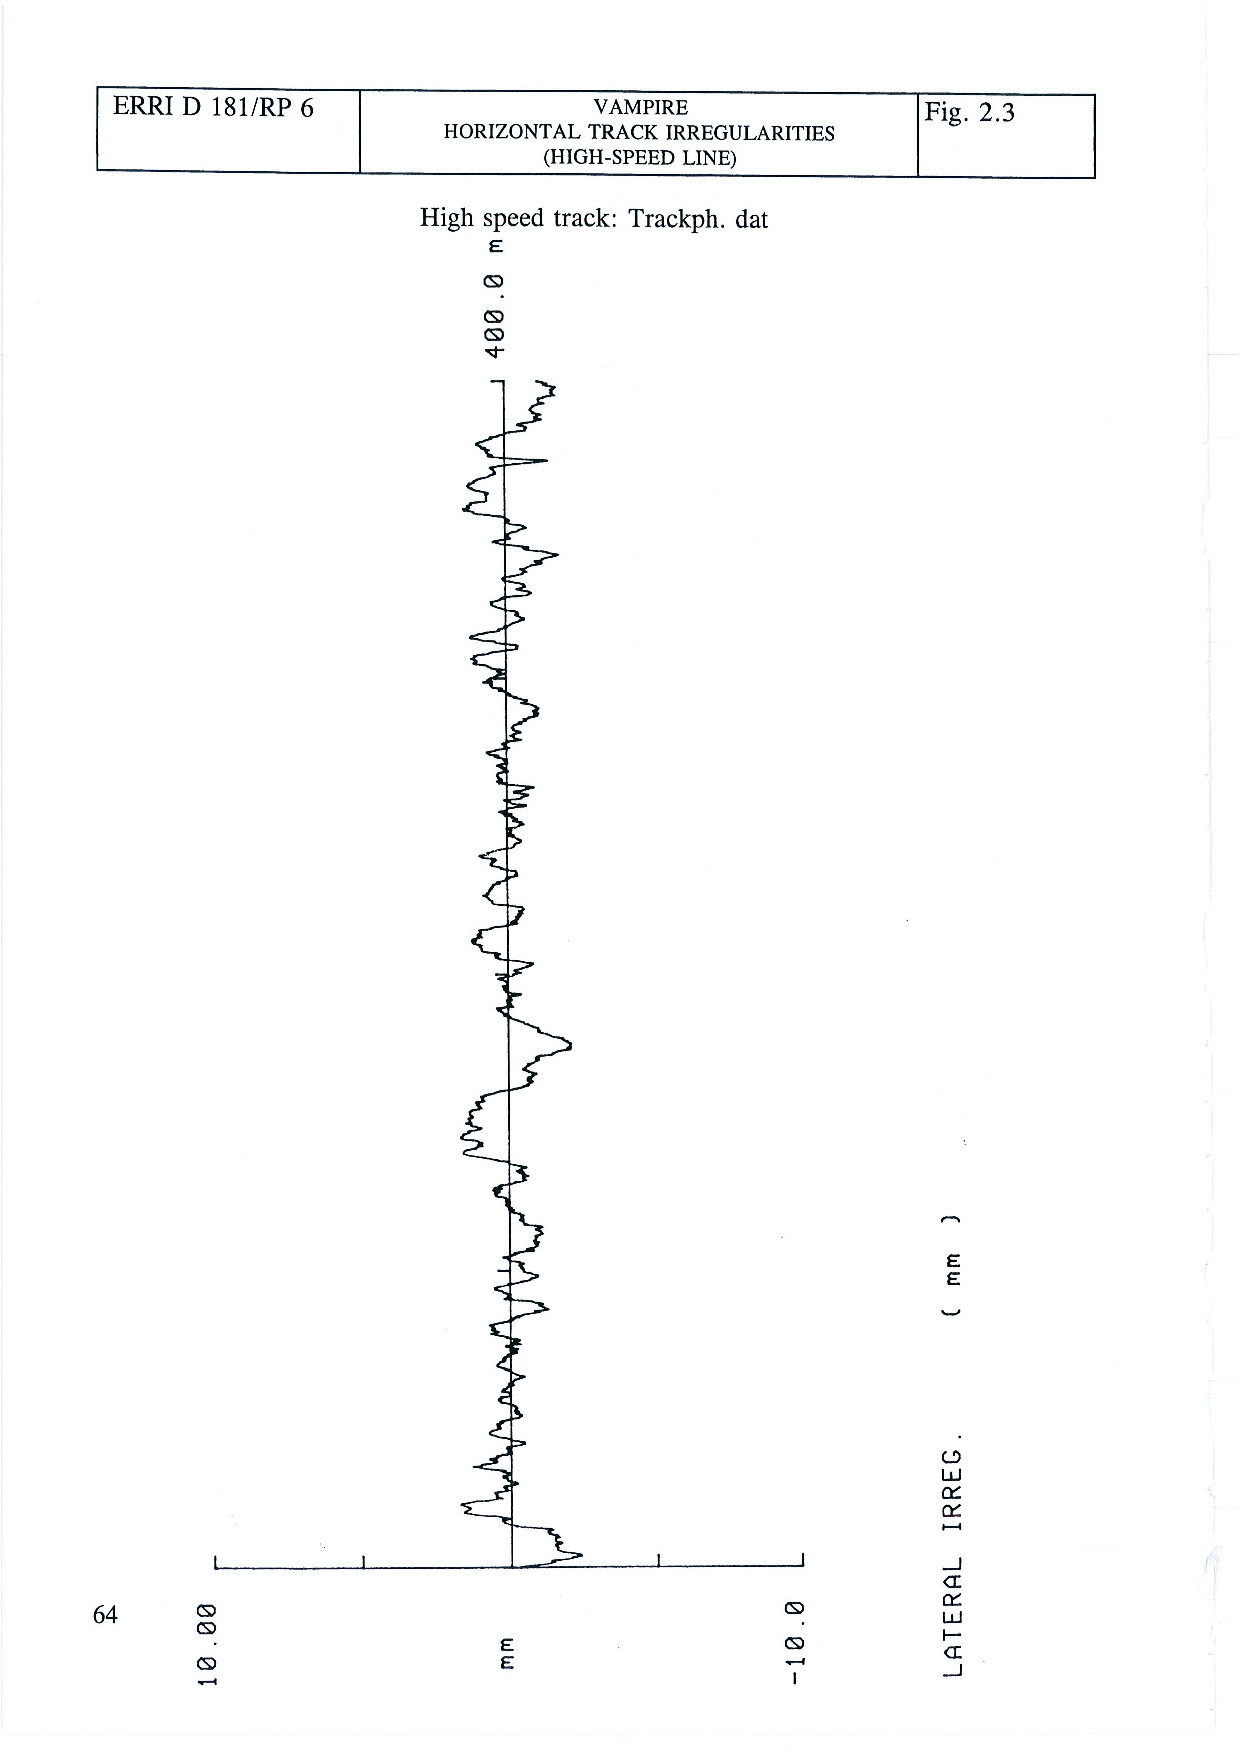
\includegraphics[width=\textwidth]{track3}
    \caption{Horizontal track irregularities for high speed passenger train. Extract from \cite[Figure 2.1]{d181}}
    \label{fig:track3}
\end{figure}

\begin{table}[h]
    \centering
    \begin{tabular}{c|c|c|c}
    \hline
    \multirow{2}{*}{Freight train: Principle axle repeat patterns} & dist & \multicolumn{2}{c}{Speed} \\
    & m & 60 km/h & 100 km/h \\
    \hline
    wagon n axle 2 - wagon n+1 axle 1 & 4.00 & 4.17 & 6.94 \\
    wagon wheelbase & 9.00 & 1.85 & 3.09 \\
    wagon n axle m - wagon n+1 axle m & 13.0 & 1.28 & 2.14 \\
    wagon n axle m - wagon n+2 axle m & 26.0 & 0.64 & 1.07 \\
    \hline
    \multirow{2}{*}{Passenger train: Principle axle repeat patterns} & dist & \multicolumn{2}{c}{Speed} \\
    & m & 160 km/h & 200 km/h \\
    \hline
    coach n axle 1 - 2, and coach n axle 3 - 4 & 2.56 & 17.36 & 21.70 \\
    coach n axle m - coach n+1 axle m & 26.4 & 1.68 & 2.10 \\
    coach n axle m - coach n+2 axle m & 52.8 & 0.84 & 1.05 \\
    \hline
    \multirow{2}{*}{ETR 500 train: Principle axle repeat patterns} & dist & \multicolumn{2}{c}{Speed} \\
    & m & 300 km/h & 350 km/h \\
    \hline
    coach n axle 1 - 2 and coach n axle 3 - 4 & 3.0 & 27.78 & 32.41 \\
    coach n axle m - coach n+1 axle m & 26.1 & 3.19 & 3.72 \\
    coach n axle m - coach n+2 axle m & 52.2 & 1.60 & 1.86 \\
    coach n axle m - coach n+3 axle m & 69.3 & 1.20 & 1.40 \\
    \hline
    \end{tabular}
    \caption{Axle repeat patterns and typical frequencies. Extracted from \cite[Appendix C]{d181dt329}}
    \label{tab:329axlerepeat}
\end{table}

\begin{table}[h]
    \centering
    \begin{tabular}{c|c|c|c}
    \hline
    Kinematic wavelength, m & Freight train & Passenger train & ETR500 train \\
    \hline
    Locomotive & 39 - 45 & 32 - 38 & 39 - 45 \\
    Coach/wagon & 24 - 39 & 34 - 38 & 36 - 40 \\
    \hline
    \end{tabular}
    \caption{Kinematic wavelength ranges per vehicle, with BR P1 profiles. Extracted from \cite[Appendix C]{d181dt329}}
    \label{tab:329kinematicwavelength}
\end{table}

\chapter{Speeds which do not require dynamic compatibility checks} \label{app:speedsafe}

\begin{figure}[h]
    \centering
    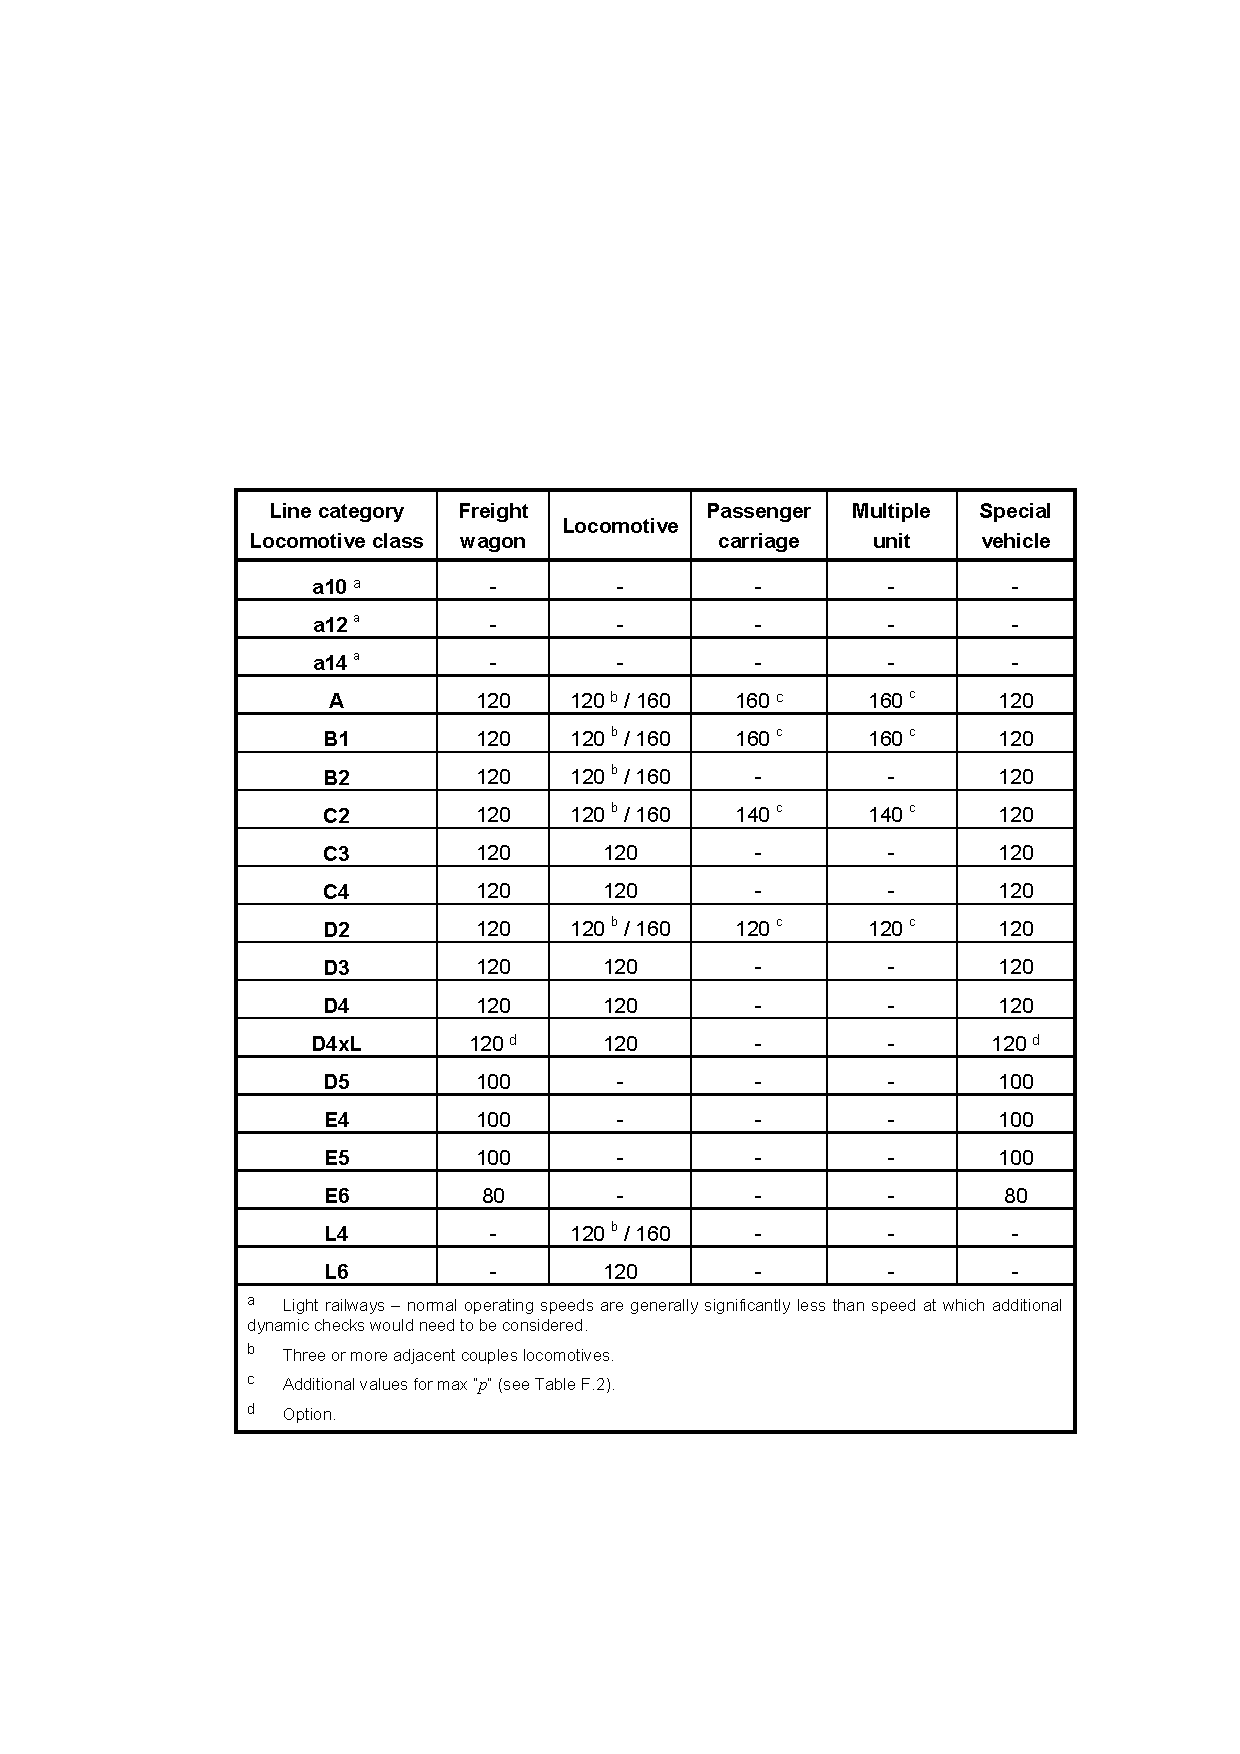
\includegraphics[width=0.7\textwidth]{speedsafe.pdf}
    \caption{Speed limit (in km/h) in relationship Line Category/Locomotive Class and vehicle type. Extract from \cite[Appendix F]{EC15528}}
\end{figure}


\begin{figure}[h]
    \centering
    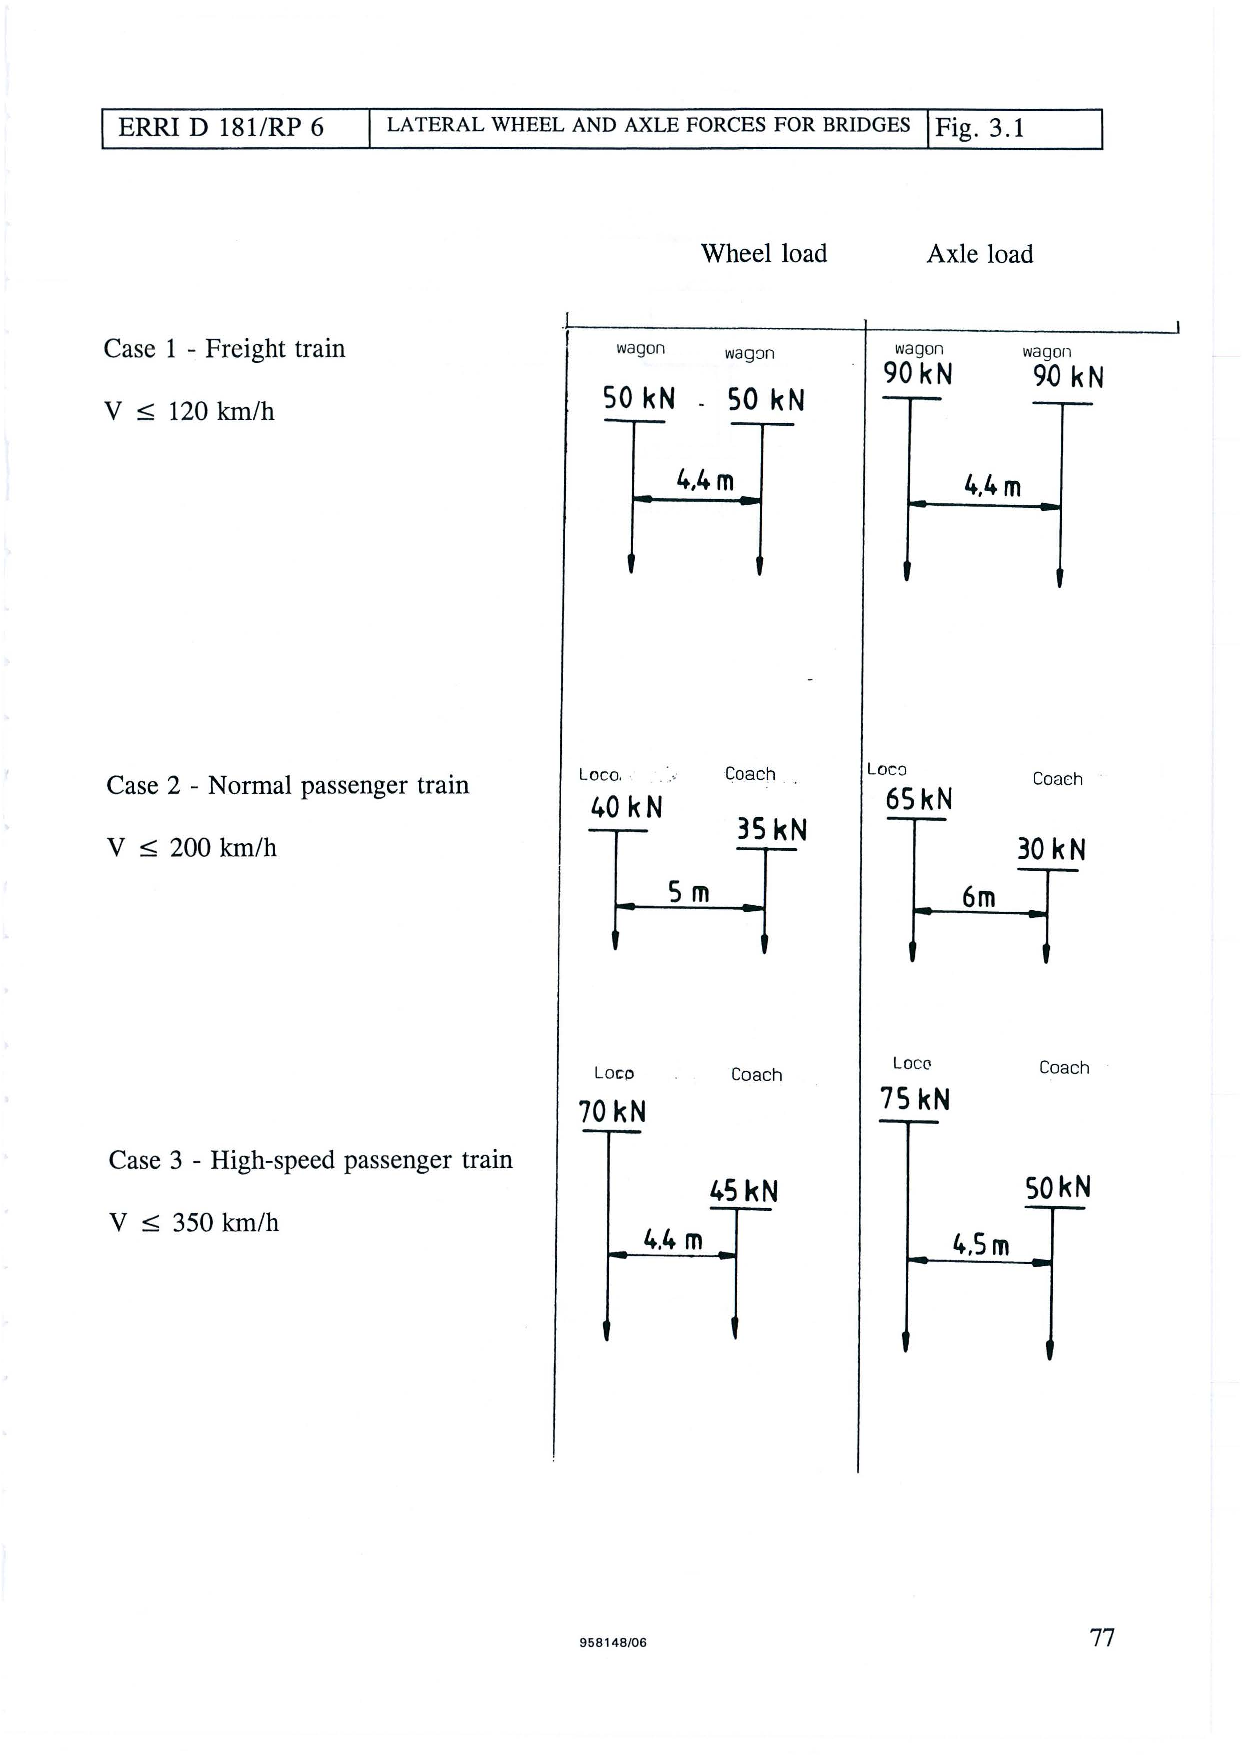
\includegraphics[width=\textwidth]{lateralloadcasesample}
    \caption{LATERAL WHEEL AND AXLE FORCES FOR BRIDGES. Extract from \cite[Fig 3.1]{d181}}
    \label{fig:lateralloadcasesample}
\end{figure}

\begin{figure}[h]
    \centering
    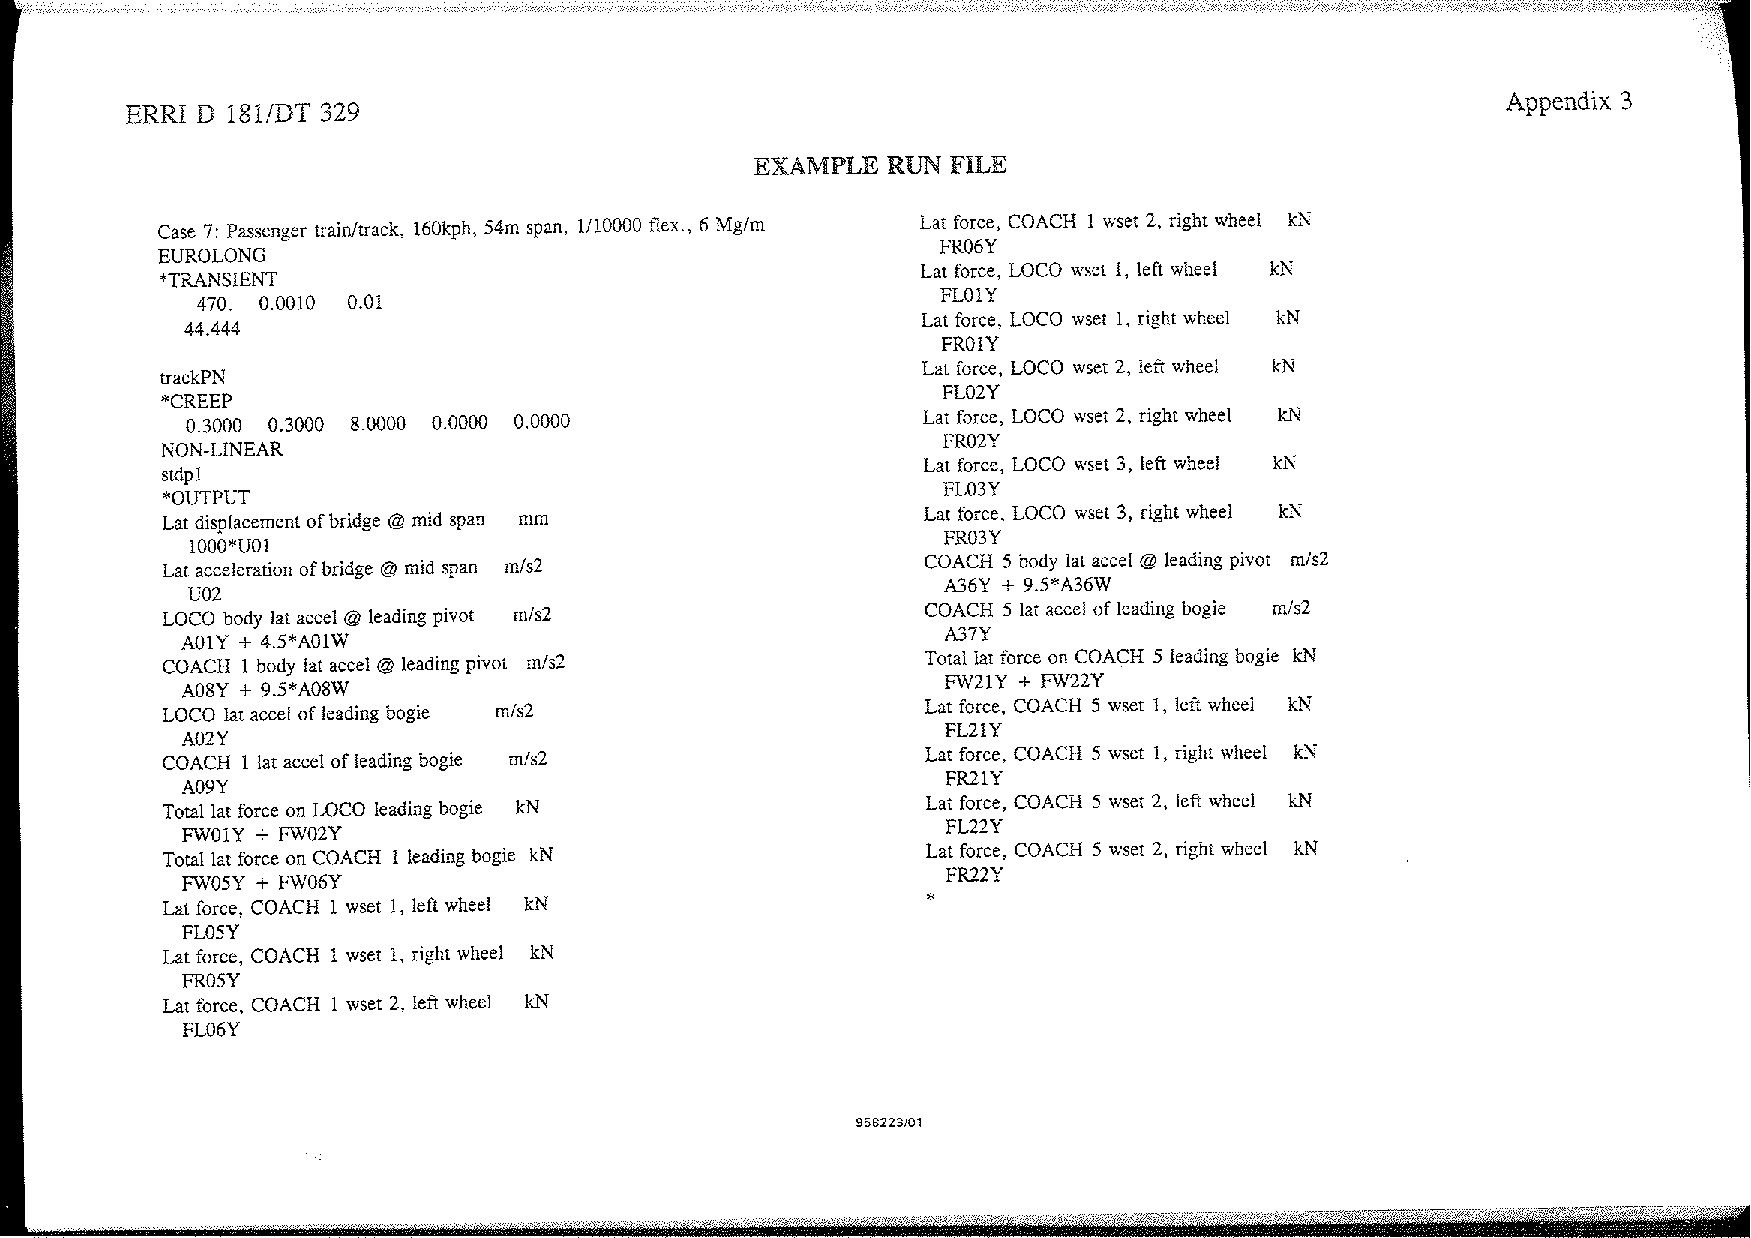
\includegraphics[width=\textwidth]{examplerunfile}
    \caption{Example run file. Extracted from \cite{d181dt329}.  }
    \label{fig:examplerunfile}
\end{figure}

\chapter{MU-Groups and MU-Classes}\label{app:mu}

\section{Definition}
Multiple units can be grouped according to type of traffic service(high speed - long distance, intercity - regional and commuter/suburban) or to the kind of running gear (conventional bogies, articulated bogies and single axles).


In some cases due to potential excessive dynamic load effects in bridge line category checks are not sufficient to demonstrate compatibility. To minimise the need for undertaking a dynamic check of individual trains, several typical and wide spread MU-designs have been grouped in MU-classes. For these groups of vehicles, load models covering the specified design parameter ranges have been developed to allow the efficient dynamic analysis of bridges. For practical reasons, the number of MU classes was limited and for trains outside the range of parameters covered, the process of checking an individual train existing at the time of publication of this standard as state of the art shall be used.

Each MU-class is defined by:

\begin{enumerate}[-]
\item ranges of train parameters covered and;
\item a corresponding load model for carrying out dynamic checks on bridges.
\end{enumerate}

Each MU-Group comprises of serveral MU-Classes. Table

\begin{table}[h]
    \centering
    \begin{tabular}{c|c}
        \hline
        MU-Group & MU-Class\\
        \hline
        \multirow{2}{*}{conventional bogie(CB)} & $CB_1$ \\
        & $CB_2$ \\
        \hline
        \multirow{4}{*}{articulated bogie(AB)} & $AB_1$ \\
        & $AB_2$ \\
        & $AB_3$ \\
        & $AB_4$ \\
        \hline
        \multirow{2}{*}{single axle(SA)} & $SA_1$ \\
        & $SA_2$ \\
        \hline
    \end{tabular}
    \caption{Relationship MU-groups - MU-classes}
    \label{tab:MU}
\end{table} 

\begin{figure}[h]
\centering
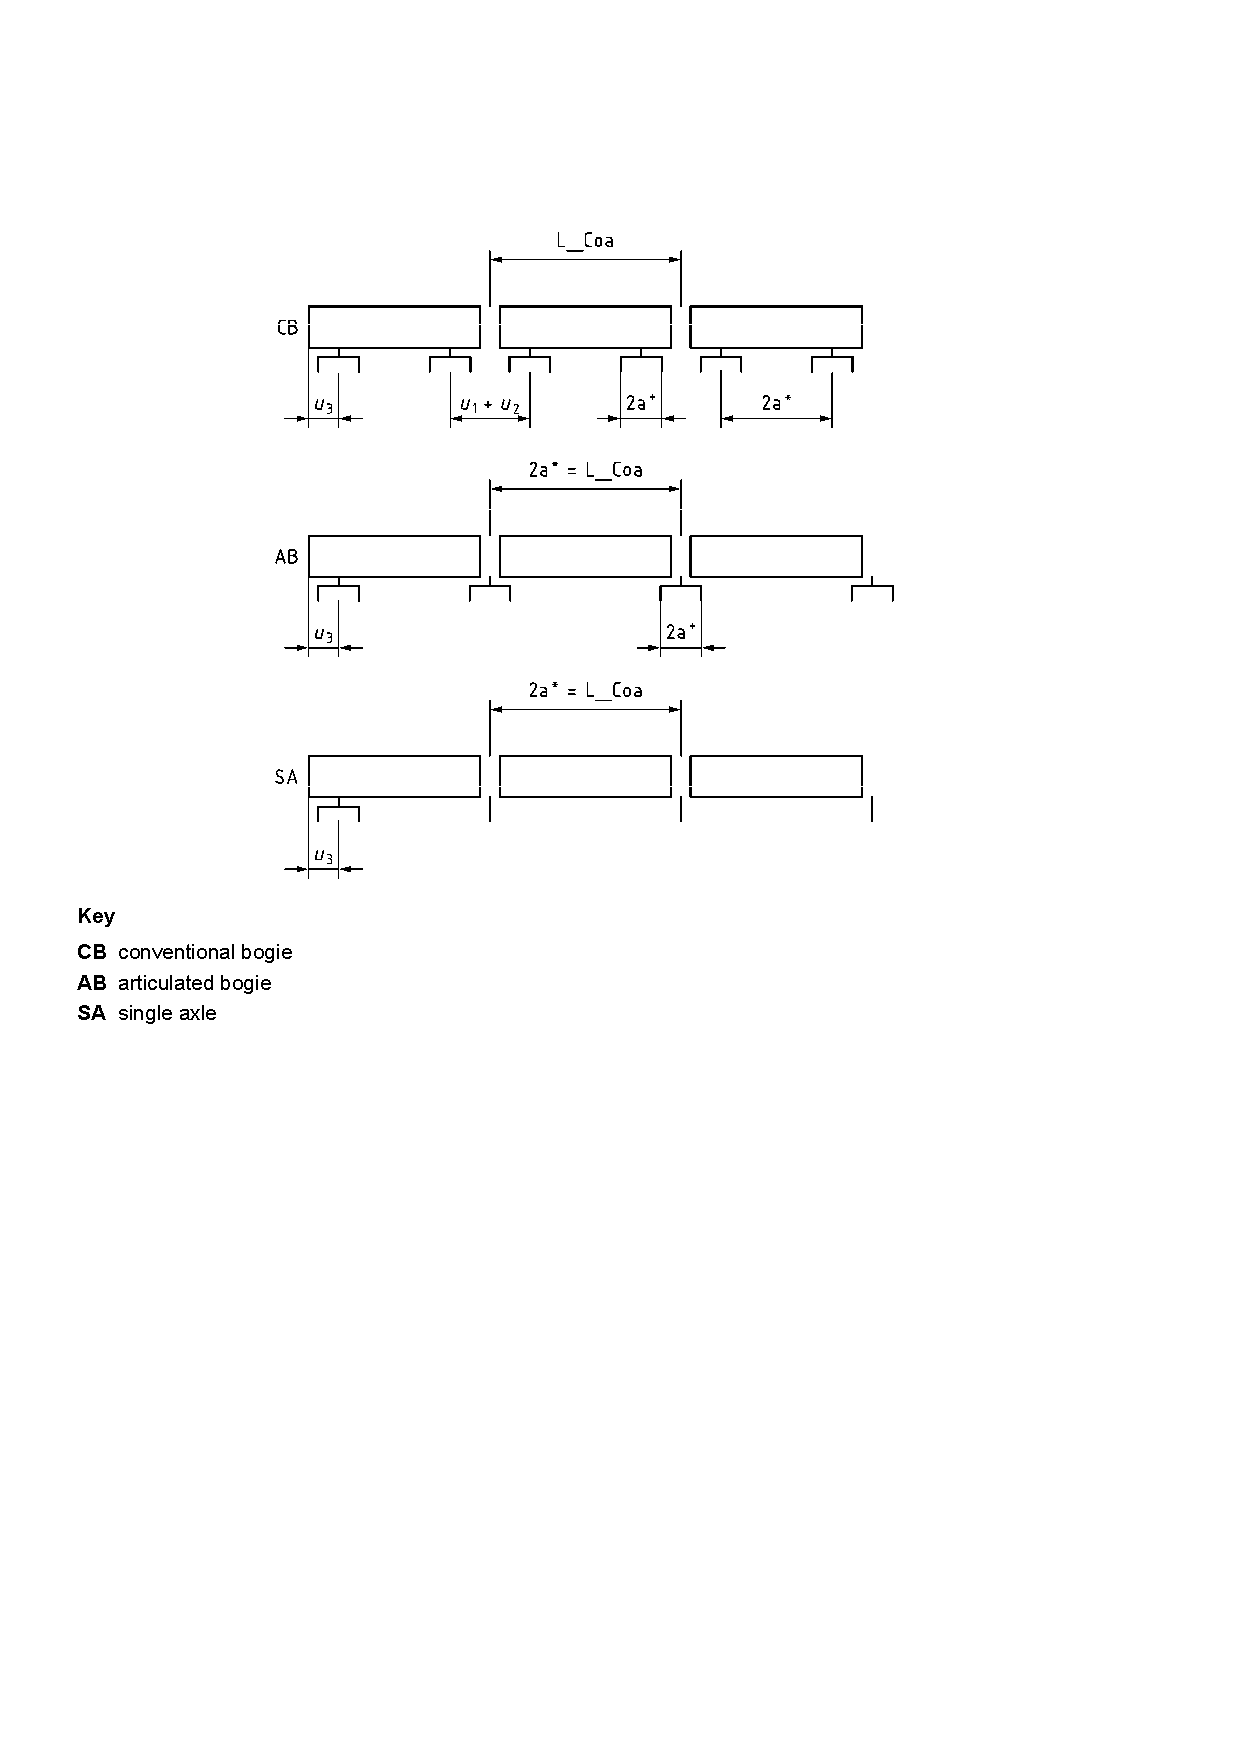
\includegraphics[width=0.8\textwidth]{trainparameters.pdf}
\caption{Train parameters related to MU-Groups. Extracted from \cite[Annex C]{EC15528}}
\label{fig:trainparameters}
\end{figure}

\begin{table}[h]
    \centering
    \begin{tabular}{c|c|c}
    \hline
    Name & Parameter & Unit \\
    $2a^*$ & Bogie spacing between pivot centres within a vehicle & m \\
    $2a^+$ & Axle spacing in bogie & m \\
    $u1+u2$ & Bogie spacing between pivot centres of adjacent vehicles & m \\
    $u3$ & Overhang of end coaches & m \\
    L\_Coa & Coach length & m \\
    No\_Coa & Number of coaches within an unit & - \\
    No\_Units & Number of units within a train & - \\
    \hline
    \end{tabular}
    \caption{Explanation of train parameters. Extracted from \cite[Annex C]{EC15528}}
    \label{tab:explanationtrainparameters}
\end{table}

\subsection{Train parameters of MU-Class CB\_1}

\begin{table}[h]
    \centering
    \begin{tabular}{c|c}
    \hline
    max No\_Units & 2 \\
    max No\_Coa & 8 \\
    L\_Coa & $23.8m \leq L\_Coa \leq 25.3m $ \\
    $2a^*$ & $16.8m \leq 2a^* \leq 18.0m $ \\
    $2a^+$ & $2m \leq 2a^+ \leq 3m $ \\
    $(u1+u2)$ & $7.0m \leq (u1+u2) \leq 7.6m $ \\
    $u3$ & $4m \leq u3 \leq 6m $ \\
    \hline
    \end{tabular}
    \caption{Train parameters for conformity with MU-Class CB\_1}
    \label{tab:CB1}
\end{table}

\subsection{Train parameters of MU-Class CB\_2}

\begin{table}[h]
    \centering
    \begin{tabular}{c|c}
    \hline
    max No\_Units & 2 \\
    max No\_Coa & 7 \\
    L\_Coa & $ 25.3 m \leq L\_Coa \leq 27.5 m $ \\
    $2a^*$ & $ 18.0 m \leq 2a^* \leq 19.5 m $ \\
    $2a^+$ & $ 2 m \leq 2a^+ \leq 3m $ \\
    $(u1+u2)$ & $7.2m \leq (u1+u2) \leq 8.0 m $ \\
    $u3$ & $4m \leq u3 \leq 6m $ \\
    \hline
    \end{tabular}
    \caption{Train parameters for conformity with MU-Class CB\_2}
    \label{tab:CB2}
\end{table}


\subsection{Train parameters of MU-Class AB\_1}

\begin{table}[h]
    \centering
    \begin{tabular}{c|c}
    \hline
    max No\_Units & 4 \\
    max No\_Coa & 5 \\
    $2a^*$ & $ 14.9 m \leq 2a^* \leq 16.0 m $ \\
    $2a^+$ & $ 2 m \leq 2a^+ \leq 3m $ \\
    $u3$ & $3m \leq u3 \leq 5.5m $ \\
    \hline
    \end{tabular}
    \caption{Train parameters for conformity with MU-Class AB\_1}
    \label{tab:AB1}
\end{table}

\subsection{Train parameters of MU-Class AB\_2}

\begin{table}[h]
    \centering
    \begin{tabular}{c|c}
    \hline
    max No\_Units & 4 \\
    max No\_Coa & 5 \\
    $2a^*$ & $ 18.8 m \leq 2a^* \leq 19.5 m $ \\
    $2a^+$ & $ 2 m \leq 2a^+ \leq 3m $ \\
    $u3$ & $3m \leq u3 \leq 5.5m $ \\
    \hline
    \end{tabular}
    \caption{Train parameters for conformity with MU-Class AB\_2}
    \label{tab:AB2}
\end{table}

\subsection{Train parameters of MU-Class AB\_3}

\begin{table}[h]
    \centering
    \begin{tabular}{c|c}
    \hline
    max No\_Units & 2 \\
    max No\_Coa & 11 \\
    $2a^*$ & $ 17.0 m \leq 2a^* \leq 17.5 m $ \\
    $2a^+$ & $ 2 m \leq 2a^+ \leq 3m $ \\
    $u3$ & $4.5m \leq u3 \leq 5.7m $ \\
    \hline
    \end{tabular}
    \caption{Train parameters for conformity with MU-Class AB\_3}
    \label{tab:AB3}
\end{table}

\subsection{Train parameters of MU-Class AB\_4}

\begin{table}[h]
    \centering
    \begin{tabular}{c|c}
    \hline
    max No\_Units & 2 \\
    max No\_Coa & 10 \\
    $2a^*$ & $ 18.7 m \leq 2a^* \leq 19.2 m $ \\
    $2a^+$ & $ 2 m \leq 2a^+ \leq 3m $ \\
    $u3$ & $4.3m \leq u3 \leq 5.3m $ \\
    \hline
    \end{tabular}
    \caption{Train parameters for conformity with MU-Class AB\_4}
    \label{tab:AB4}
\end{table}

\subsection{Train parameters of MU-Class SA\_1}

\begin{table}[h]
    \centering
    \begin{tabular}{c|c}
    \hline
    max No\_Units & 3 \\
    max No\_Coa & 10 \\
    $2a^*$ & $ 9.2 m \leq 2a^* \leq 9.8 m $ \\
    $u3$ & $4.25m \leq u3 \leq 6.25m $ \\
    \hline
    \end{tabular}
    \caption{Train parameters for conformity with MU-Class SA\_1}
    \label{tab:SA1}
\end{table}

\subsection{Train parameters of MU-Class SA\_2}

\begin{table}[h]
    \centering
    \begin{tabular}{c|c}
    \hline
    max No\_Units & 2 \\
    max No\_Coa & 14 \\
    $2a^*$ & $ 12.8 m \leq 2a^* \leq 13.5 m $ \\
    $u3$ & $4.25m \leq u3 \leq 6.25m $ \\
    \hline
    \end{tabular}
    \caption{Train parameters for conformity with MU-Class SA\_1}
    \label{tab:SA1}
\end{table}

\chapter{Regression commands for R console}\label{sec:Rregression}

\begin{lstlisting}[keywordstyle=\bfseries\color{blue},language=R]
> F <- c(0,110,170,185)
> v <- c(0,60,100,120)
> f <- function(a,b,v) {a*v^b}
> dat <- data.frame(v,F)
> dat
    v   F
1   0   0
2  60 110
3 100 170
4 120 185

> fm <- nls(F ~ f(a,b,v), data = dat, start = c(a=1, b=1))
> fm
Nonlinear regression model
  model: F ~ f(a, b, v)
   data: dat
     a      b 
5.2064 0.7498 
 residual sum-of-squares: 47.84

Number of iterations to convergence: 6 
Achieved convergence tolerance: 2.868e-06
\end{lstlisting}

\chapter{Matlab scripts}\label{sec:matlabscripts}
\section{fog.m}
\lstinputlisting{./matlab/fog.m}
\section{Speedenvelop.m}
\lstinputlisting{./matlab/Speedenvelop.m}
\section{Spanenvelop.m}
\lstinputlisting{./matlab/Spanenvelop.m}
\section{Stiffenvelop.m}
\lstinputlisting{./matlab/Stiffenvelop.m}
\section{Massenvelop.m}
\lstinputlisting{./matlab/Massenvelop.m}


\chapter{Train vehicles}

\section{Locomotives}
\subsection{4-axle locomotives}
Generally, the relevant parameters for categorisation of 4-axle locomotives are axle load P (18 t to 22,5 t) and the bogie axle spacing (2,2 m to 3,4 m).

Typically the mass per unit length is less than 6,4 t/m and the distance from the end axle to the end of the nearest coupling plane is greater than 1,9 m

\subsection{6-axle locomotives}

Generally, the relevant parameters for categorisation of 6-axle locomotives are:

\begin{enumerate}[-]
\item the maximum axle load P (18 t to 22 t) in combination with;
\item the distance between axles within a bogie (1,80 m to 2,25 m).
\end{enumerate}

Typically, the mass per unit length (p) is less than 6,4 t/m and the distance from end axle to the end of the nearest coupling plane (a) is greater than 2,1 m.

\section{Trains in Netherlands}

Passenger trains now in service include following models:

\begin{enumerate}
    \item The DD-AR (Dubbeldeksaggloregiomaterieel) \\  EMUs were delivered as DDM-2/3 resembling the bilevel rail cars series DDM-1 from 1985 and operates in fixed formations of 3 or 4 coaches. 4 car trains use a class 1700 locomotive for traction, 3 car trains use an mDDM motorcar, which resembles a DD-AR driving trailer but has electric motors and a single passenger deck on top; the level of this deck is higher than that of a regular single deck rail car, but lower than the upper deck of the other coaches. Three types of coaches are available: Bv (second class), ABv (first and second class) and Bvk (second class driving trailer). The DDM-2/3 series are being modernised from 2010–2013 and after modernisation the series was renamed as NID (Nieuwe Intercity Dubbeldekker).
    \item The VIRM (Verlengd Interregiomaterieel) \\ also called Regiorunner was partially rebuilt from trainsets DD-IRM (Dubbeldeks Interregiomaterieel). DD-IRM was delivered in 3- and 4-car trainsets. 3-car trainsets got one extra coach, 4-car trainsets got two extra coaches. Also, new 4- and 6-car trainsets were built. Thus, a train consists of one or more combinations of 4 or 6 double deck coaches; each combination (multiple unit) has electric motors. More than three hundred coaches are currently operative in the Netherlands.
    \item The Koploper (ICM) (Intercitymaterieel) \\ is a 3- or 4-car multiple unit that when coupled with another one, allows passengers to walk through (the name Koploper being a play on words – literally "head walker", but in actual use meaning "front runner"). The Dutch Railway Company decided to close the heads permanently on 31 October 2005 because the mechanism broke down too often. A scheduled modernisation of around 7 million euro will see the ICM fleet updated. The renovated ICM trains provide 13\% more seats (reducing the leg room to uncomfortable small for the long haul journeys they serve in 2nd class, which is further aggravated by a waste bin that is placed on the backsides of the seats in front), have a new interior, a bathroom accessible by wheelchairs, airconditioning as well as upgrades to the engine and connection systems. The head doors are removed. Also, these (renovated) trains are the first trains in the NS fleet equipped with OBIS. OBIS provides a (free) WiFi-connection on board, along with in-train journey information provided through screens and (automated) vocal announcements through the trains speakers. This journey information provides the actual status, and thus is always up-to-date to the actual situation this trip, and the stations is passes.
    \item The Sprinter (SGM, Stads Gewestelijk Materieel) \\ is a two or three car electric, used on small distances. They are named Sprinter because they're able to accelerate and brake quite fast, making them very suitable for 'stoptrein' services. They were also specifically designed for urban environments where they run commuter services. As a result, they are most commonly found in the Randstad area. The initial idea was that the Sprinter would provide somewhat of a subway/metro service but this plan failed as the cities of Amsterdam and Rotterdam continued to construct their own rapid transit systems. Nevertheless, in the densely populated Randstad, the Sprinters remain popular. Two car versions were revised and renamed to Citypendel. All Sprinters are now refurbished into the new white/yellow/dark blue livery.
\end{enumerate}
\end{appendices}